\documentclass[11pt,a4paper]{article}
\usepackage[margin=24mm]{geometry}
\usepackage[T1]{fontenc}
\usepackage[utf8]{inputenc}
\usepackage[british]{babel}
\usepackage{lmodern,microtype,amsmath,amssymb,booktabs,tabularx,graphicx,array}
\usepackage{xcolor,caption,placeins,textcomp}
\definecolor{ink}{HTML}{243340}
\definecolor{figteal}{HTML}{007F86}
\definecolor{light}{HTML}{F2F5F7}
\usepackage[colorlinks=true,linkcolor=figteal,citecolor=figteal,urlcolor=figteal]{hyperref}
\hypersetup{pdftitle={Causality and symbolic computation: from Boolean networks to a compiler},pdfauthor={Alberto Hern\'andez-Espinosa}}
\captionsetup{font=small,labelfont=bf}
\setlength{\parskip}{3pt}
\setlength{\emergencystretch}{3em}
\graphicspath{{generated/}}
\makeatletter
\newcommand{\tableinput}[1]{\@@input #1 }
\makeatother
% Generated by phase2_evidence.Ledger. Do not edit.
\makeatletter
\expandafter\def\csname lv@bA\endcsname{0.01}
\expandafter\def\csname lv@bB\endcsname{0.1}
\expandafter\def\csname lv@bC\endcsname{1}
\expandafter\def\csname lv@exAchosen\endcsname{2}
\expandafter\def\csname lv@exAddrBits\endcsname{8}
\expandafter\def\csname lv@exAhi\endcsname{2}
\expandafter\def\csname lv@exBoxCcap\endcsname{7}
\expandafter\def\csname lv@exBoxClosed\endcsname{7}
\expandafter\def\csname lv@exBoxLC\endcsname{8}
\expandafter\def\csname lv@exBoxLS\endcsname{3}
\expandafter\def\csname lv@exBoxPolicy\endcsname{k4 memory}
\expandafter\def\csname lv@exBoxScap\endcsname{2}
\expandafter\def\csname lv@exCatalogue\endcsname{17}
\expandafter\def\csname lv@exCerts\endcsname{15,137}
\expandafter\def\csname lv@exClC\endcsname{9}
\expandafter\def\csname lv@exClJ\endcsname{45}
\expandafter\def\csname lv@exClPeakCycle\endcsname{4}
\expandafter\def\csname lv@exClPrio\endcsname{6}
\expandafter\def\csname lv@exClS\endcsname{5}
\expandafter\def\csname lv@exClStoreA\endcsname{7}
\expandafter\def\csname lv@exClStoreB\endcsname{8}
\expandafter\def\csname lv@exCodeMax\endcsname{31}
\expandafter\def\csname lv@exEpochs\endcsname{1}
\expandafter\def\csname lv@exHorizon\endcsname{21}
\expandafter\def\csname lv@exHorizonLast\endcsname{20}
\expandafter\def\csname lv@exLatSum\endcsname{3+3+3+3+2+2+1+1+1+1+1}
\expandafter\def\csname lv@exMaxCover\endcsname{4}
\expandafter\def\csname lv@exNodes\endcsname{366}
\expandafter\def\csname lv@exOps\endcsname{11}
\expandafter\def\csname lv@exOptCmax\endcsname{11}
\expandafter\def\csname lv@exOptJm\endcsname{23}
\expandafter\def\csname lv@exOptSchedules\endcsname{24,142}
\expandafter\def\csname lv@exOursC\endcsname{8}
\expandafter\def\csname lv@exOursJ\endcsname{24}
\expandafter\def\csname lv@exOursPeakCycle\endcsname{4}
\expandafter\def\csname lv@exOursS\endcsname{3}
\expandafter\def\csname lv@exOursStoreA\endcsname{6}
\expandafter\def\csname lv@exOursStoreB\endcsname{7}
\expandafter\def\csname lv@exQaA\endcsname{1*000}
\expandafter\def\csname lv@exQaB\endcsname{01000}
\expandafter\def\csname lv@exQaC\endcsname{*0100}
\expandafter\def\csname lv@exQaD\endcsname{01100}
\expandafter\def\csname lv@exQanchors\endcsname{1, 2, 4 and 6}
\expandafter\def\csname lv@exQbA\endcsname{**000}
\expandafter\def\csname lv@exQbB\endcsname{*0100}
\expandafter\def\csname lv@exQbC\endcsname{01100}
\expandafter\def\csname lv@exQhi\endcsname{6}
\expandafter\def\csname lv@exQlen\endcsname{7}
\expandafter\def\csname lv@exQueries\endcsname{20}
\expandafter\def\csname lv@exRatioCl\endcsname{1.875}
\expandafter\def\csname lv@exRatioSer\endcsname{4.5}
\expandafter\def\csname lv@exRootClosed\endcsname{8}
\expandafter\def\csname lv@exSearched\endcsname{2}
\expandafter\def\csname lv@exSerC\endcsname{12}
\expandafter\def\csname lv@exSerJ\endcsname{108}
\expandafter\def\csname lv@exSerLast\endcsname{11}
\expandafter\def\csname lv@exSerS\endcsname{9}
\expandafter\def\csname lv@exTimeBits\endcsname{5}
\expandafter\def\csname lv@exValues\endcsname{9}
\expandafter\def\csname lv@exWholeCcap\endcsname{21}
\expandafter\def\csname lv@exWholeLC\endcsname{7}
\expandafter\def\csname lv@exWholeLS\endcsname{1}
\expandafter\def\csname lv@exWholeNodes\endcsname{186}
\expandafter\def\csname lv@exWholeScap\endcsname{3}
\expandafter\def\csname lv@exWinD\endcsname{9}
\expandafter\def\csname lv@lvOne\endcsname{98.33}
\expandafter\def\csname lv@lvThree\endcsname{97.5}
\expandafter\def\csname lv@mPublic\endcsname{8}
\expandafter\def\csname lv@mVlen\endcsname{8}
\expandafter\def\csname lv@mWords\endcsname{256}
\expandafter\def\csname lv@pOneScore\endcsname{2.008466}
\expandafter\def\csname lv@rOneClHi\endcsname{12.84}
\expandafter\def\csname lv@rOneClLo\endcsname{8.38}
\expandafter\def\csname lv@rOneClRed\endcsname{10.58}
\expandafter\def\csname lv@rOneClTime\endcsname{76.20}
\expandafter\def\csname lv@rOneCllosses\endcsname{20}
\expandafter\def\csname lv@rOneClties\endcsname{42}
\expandafter\def\csname lv@rOneClwins\endcsname{138}
\expandafter\def\csname lv@rTwoDfsClL\endcsname{15}
\expandafter\def\csname lv@rTwoDfsClRed\endcsname{14.4}
\expandafter\def\csname lv@rTwoDfsClT\endcsname{39}
\expandafter\def\csname lv@rTwoDfsClW\endcsname{146}
\expandafter\def\csname lv@rTwoPubClassical\endcsname{1.901379}
\expandafter\def\csname lv@resident\endcsname{8}
\expandafter\def\csname lv@rpBetter\endcsname{7}
\expandafter\def\csname lv@rpC1CallMed\endcsname{100.7}
\expandafter\def\csname lv@rpC1ProcMax\endcsname{0.157}
\expandafter\def\csname lv@rpC1Runs\endcsname{40}
\expandafter\def\csname lv@rpClCallMed\endcsname{0.269}
\expandafter\def\csname lv@rpCycBetter\endcsname{2}
\expandafter\def\csname lv@rpCycCOne\endcsname{1.444}
\expandafter\def\csname lv@rpCycCl\endcsname{1.494}
\expandafter\def\csname lv@rpCycWorse\endcsname{3}
\expandafter\def\csname lv@rpEqual\endcsname{1}
\expandafter\def\csname lv@rpGainPct\endcsname{15.1}
\expandafter\def\csname lv@rpJRed\endcsname{24.5}
\expandafter\def\csname lv@rpScrBetter\endcsname{7}
\expandafter\def\csname lv@rpScrCOne\endcsname{3.316}
\expandafter\def\csname lv@rpScrCl\endcsname{2.420}
\expandafter\def\csname lv@rpTmixedbroadcastCOne\endcsname{9\ensuremath{\times}16}
\expandafter\def\csname lv@rpTmixedbroadcastCOneJ\endcsname{144}
\expandafter\def\csname lv@rpTmixedbroadcastCl\endcsname{9\ensuremath{\times}17}
\expandafter\def\csname lv@rpTmixedbroadcastClJ\endcsname{153}
\expandafter\def\csname lv@rpTmixedbroadcastSer\endcsname{11\ensuremath{\times}42}
\expandafter\def\csname lv@rpTmixedbroadcastSerJ\endcsname{462}
\expandafter\def\csname lv@rpTparallelmemoryCOne\endcsname{13\ensuremath{\times}40}
\expandafter\def\csname lv@rpTparallelmemoryCOneJ\endcsname{520}
\expandafter\def\csname lv@rpTparallelmemoryCl\endcsname{14\ensuremath{\times}56}
\expandafter\def\csname lv@rpTparallelmemoryClJ\endcsname{784}
\expandafter\def\csname lv@rpTparallelmemorySer\endcsname{21\ensuremath{\times}128}
\expandafter\def\csname lv@rpTparallelmemorySerJ\endcsname{2,688}
\expandafter\def\csname lv@rpTscalardualchainCOne\endcsname{8\ensuremath{\times}3}
\expandafter\def\csname lv@rpTscalardualchainCOneJ\endcsname{24}
\expandafter\def\csname lv@rpTscalardualchainCl\endcsname{9\ensuremath{\times}5}
\expandafter\def\csname lv@rpTscalardualchainClJ\endcsname{45}
\expandafter\def\csname lv@rpTscalardualchainSer\endcsname{12\ensuremath{\times}9}
\expandafter\def\csname lv@rpTscalardualchainSerJ\endcsname{108}
\expandafter\def\csname lv@rpTscalarpipelineCOne\endcsname{14\ensuremath{\times}6}
\expandafter\def\csname lv@rpTscalarpipelineCOneJ\endcsname{84}
\expandafter\def\csname lv@rpTscalarpipelineCl\endcsname{14\ensuremath{\times}6}
\expandafter\def\csname lv@rpTscalarpipelineClJ\endcsname{84}
\expandafter\def\csname lv@rpTscalarpipelineSer\endcsname{18\ensuremath{\times}15}
\expandafter\def\csname lv@rpTscalarpipelineSerJ\endcsname{270}
\expandafter\def\csname lv@rpTscalarselectsCOne\endcsname{10\ensuremath{\times}5}
\expandafter\def\csname lv@rpTscalarselectsCOneJ\endcsname{50}
\expandafter\def\csname lv@rpTscalarselectsCl\endcsname{9\ensuremath{\times}6}
\expandafter\def\csname lv@rpTscalarselectsClJ\endcsname{54}
\expandafter\def\csname lv@rpTscalarselectsSer\endcsname{20\ensuremath{\times}16}
\expandafter\def\csname lv@rpTscalarselectsSerJ\endcsname{320}
\expandafter\def\csname lv@rpTvectoraxpyCOne\endcsname{11\ensuremath{\times}16}
\expandafter\def\csname lv@rpTvectoraxpyCOneJ\endcsname{176}
\expandafter\def\csname lv@rpTvectoraxpyCl\endcsname{10\ensuremath{\times}32}
\expandafter\def\csname lv@rpTvectoraxpyClJ\endcsname{320}
\expandafter\def\csname lv@rpTvectoraxpySer\endcsname{14\ensuremath{\times}73}
\expandafter\def\csname lv@rpTvectoraxpySerJ\endcsname{1,022}
\expandafter\def\csname lv@rpTvectorbitmixCOne\endcsname{13\ensuremath{\times}24}
\expandafter\def\csname lv@rpTvectorbitmixCOneJ\endcsname{312}
\expandafter\def\csname lv@rpTvectorbitmixCl\endcsname{10\ensuremath{\times}40}
\expandafter\def\csname lv@rpTvectorbitmixClJ\endcsname{400}
\expandafter\def\csname lv@rpTvectorbitmixSer\endcsname{16\ensuremath{\times}89}
\expandafter\def\csname lv@rpTvectorbitmixSerJ\endcsname{1,424}
\expandafter\def\csname lv@rpTvectorreductionCOne\endcsname{12\ensuremath{\times}32}
\expandafter\def\csname lv@rpTvectorreductionCOneJ\endcsname{384}
\expandafter\def\csname lv@rpTvectorreductionCl\endcsname{12\ensuremath{\times}40}
\expandafter\def\csname lv@rpTvectorreductionClJ\endcsname{480}
\expandafter\def\csname lv@rpTvectorreductionSer\endcsname{19\ensuremath{\times}137}
\expandafter\def\csname lv@rpTvectorreductionSerJ\endcsname{2,603}
\expandafter\def\csname lv@rpWorse\endcsname{0}
\expandafter\def\csname lv@sliceMs\endcsname{2}
\expandafter\def\csname lv@sliceNodes\endcsname{2,048}
\expandafter\def\csname lv@tAccCases\endcsname{277}
\expandafter\def\csname lv@tAccPrograms\endcsname{142}
\expandafter\def\csname lv@tCost\endcsname{0.574}
\expandafter\def\csname lv@tCostHi\endcsname{0.598}
\expandafter\def\csname lv@tCostLo\endcsname{0.552}
\expandafter\def\csname lv@tExportRows\endcsname{1,248}
\expandafter\def\csname lv@tNodes\endcsname{10,000}
\expandafter\def\csname lv@tParityPairs\endcsname{1,000}
\expandafter\def\csname lv@tPrograms\endcsname{200}
\expandafter\def\csname lv@tPubSixC1A\endcsname{2.135275}
\expandafter\def\csname lv@tPubSixC1B\endcsname{2.187957}
\expandafter\def\csname lv@tQual\endcsname{0.991}
\expandafter\def\csname lv@tQualHi\endcsname{0.996}
\expandafter\def\csname lv@tQualLo\endcsname{0.985}
\expandafter\def\csname lv@tReps\endcsname{5}
\expandafter\def\csname lv@tWTLBL\endcsname{6}
\expandafter\def\csname lv@tWTLBT\endcsname{871}
\expandafter\def\csname lv@tWTLBW\endcsname{123}
\expandafter\def\csname lv@weC1C\endcsname{9}
\expandafter\def\csname lv@weC1J\endcsname{144}
\expandafter\def\csname lv@weC1S\endcsname{16}
\expandafter\def\csname lv@weCapCcap\endcsname{17}
\expandafter\def\csname lv@weCapLC\endcsname{9}
\expandafter\def\csname lv@weCapLS\endcsname{8}
\expandafter\def\csname lv@weCapScap\endcsname{26}
\expandafter\def\csname lv@weCatalogue\endcsname{11}
\expandafter\def\csname lv@weClassicalC\endcsname{9}
\expandafter\def\csname lv@weClassicalJ\endcsname{153}
\expandafter\def\csname lv@weClassicalS\endcsname{17}
\expandafter\def\csname lv@weCombDeclared\endcsname{7,873,200}
\expandafter\def\csname lv@weCombRoot\endcsname{972,000}
\expandafter\def\csname lv@weDirectphase1C\endcsname{10}
\expandafter\def\csname lv@weDirectphase1J\endcsname{240}
\expandafter\def\csname lv@weDirectphase1S\endcsname{24}
\expandafter\def\csname lv@weEpochs\endcsname{4}
\expandafter\def\csname lv@weNodes\endcsname{5,476}
\expandafter\def\csname lv@weOps\endcsname{8}
\expandafter\def\csname lv@weQTchosen\endcsname{1}
\expandafter\def\csname lv@weQThi\endcsname{7}
\expandafter\def\csname lv@weQTlo\endcsname{0}
\expandafter\def\csname lv@weQTop\endcsname{2}
\expandafter\def\csname lv@weRootCerts\endcsname{5}
\expandafter\def\csname lv@weSerialC\endcsname{11}
\expandafter\def\csname lv@weSerialJ\endcsname{462}
\expandafter\def\csname lv@weSerialS\endcsname{42}
\expandafter\def\csname lv@weStepAC\endcsname{10}
\expandafter\def\csname lv@weStepAS\endcsname{17}
\expandafter\def\csname lv@weStepBC\endcsname{9}
\expandafter\def\csname lv@weStepBS\endcsname{17}
\expandafter\def\csname lv@weStepCC\endcsname{9}
\expandafter\def\csname lv@weStepCS\endcsname{16}
\expandafter\def\csname lv@weTimeClassical\endcsname{0.154}
\newcommand{\V}[1]{\ifcsname lv@#1\endcsname\csname lv@#1\endcsname\else\PackageError{ledger}{Undefined ledger value #1}{}\fi}
\makeatother
 
\newcommand{\ci}[2]{[#1,\,#2]}
\newcommand{\keybox}[1]{\par\smallskip\noindent\colorbox{light}{\parbox{\dimexpr\linewidth-2\fboxsep}{\small #1}}\par\smallskip}

\title{An Application of Causality and symbolic computation\\[4pt]
\large from Boolean networks to a compiler}
\author{Alberto Hern\'andez-Espinosa}
\date{September 2026}

\begin{document}
\maketitle

\begin{abstract}
The Luminal challenge asks for a compiler backend that schedules a straight-line
program on a small VLIW machine and places its values in a shared scratchpad, so
that the program runs in as few cycles and as few scratch words as possible. We
answer it with two compilers. The first is a strong \emph{classical} solution,
critical-path list scheduling followed by first-fit allocation, which we treat as
our benchmark. The second is the compiler we propose, which takes a causal view of
the problem: it asks which few decisions are responsible for the current cost,
reopens exactly those decisions, and solves them again exactly, keeping a checkable
reason for every option it rules out. On the eight public programs the classical
compiler scores \V{rTwoPubClassical} and ours \V{tPubSixC1B}, a gain of
\V{rpGainPct}\%, against the serial baseline's score of one. Ours is better on
\V{rpBetter} programs and equal on \V{rpEqual}, and it is correct on every supplied
case. The gain comes from memory: it reduces scratch by \V{rpScrCOne} times against
the classical \V{rpScrCl} times, while giving up a little in cycles
(\V{rpCycCOne} against \V{rpCycCl} times). The price is compile time: our compiler
spends its budget of \V{bB}\,s, where the classical one needs well under a
millisecond; both are far inside the grader's allowance of 20\,s.
\end{abstract}

\keybox{\textbf{The answer in four lines.}
(1)~\emph{Baseline}: the serial compiler, score one by definition.
(2)~\emph{Classical benchmark}: critical-path list scheduling and aligned first-fit
allocation, score \V{rTwoPubClassical}.
(3)~\emph{Our proposal}: build a correct first answer from exact queries, then
repeatedly reopen the decisions that cause the cost and re-solve them exactly,
score \V{tPubSixC1B}.
(4)~\emph{Trade-off}: \V{rpGainPct}\% higher score and \V{rpJRed}\% lower
geometric-mean $C\times S$ than classical, paid for with roughly \V{bB}\,s of
compilation per program.}

\section{The problem in one page}\label{sec:problem}

Luminal builds compilers for AI inference, where performance depends on how
tightly work is packed in time and how little memory it occupies while it
waits~\cite{talent}. The take-home challenge~\cite{luminal} is a small, exact
version of that problem. A program is a list of operations in dependency order:
loads, scalar and vector arithmetic, selects and stores. The machine issues one
\emph{bundle} per cycle, and each bundle may contain up to two load, two scalar and
two vector operations, one store and one flow operation. An operation's result can
be read only after its \emph{latency}: one cycle for an add, three for a scalar
load, four for a vector load. Every result lives in a scratchpad of 256 words of
32 bits; vectors take eight consecutive words starting at a multiple of eight. Two
values may share words only if their lifetimes do not overlap.

The compiler must decide two things for every operation: \emph{when} it issues
(its cycle) and \emph{where} its result lives (its scratch address). Two numbers
measure the result: the number of cycles $C$, and the footprint $S$, the highest
scratch word used. The score compares both with a frozen serial compiler,
\begin{equation}\label{eq:score}
\text{score}=\sqrt{\;\underbrace{\operatorname{geomean}_p\frac{C^{\text{serial}}_p}{C_p}}_{\text{cycle speedup}}\;\times\;
\underbrace{\operatorname{geomean}_p\frac{S^{\text{serial}}_p}{S_p}}_{\text{scratch reduction}}\;} ,
\end{equation}
so time and memory weigh exactly the same. For a single program, improving the
score is the same as reducing the product
\begin{equation}\label{eq:j}
J = C\times S .
\end{equation}
This observation shapes our whole approach: a cycle saved and a proportional amount
of scratch saved are worth the same, so a good compiler should be willing to trade
one for the other whenever the product falls.

The two decisions pull against each other. Packing a schedule tightly makes many
values alive at once, which raises $S$; packing memory tightly forces values to wait
for each other, which raises $C$. This coupling is what makes the problem
interesting, and it is where a greedy compiler leaves the most on the table.

\section{Three compilers, three ideas}\label{sec:three}

\paragraph{A program small enough to watch.} To show how a compiler actually
decides, we follow one public program of the challenge, \texttt{02\_scalar\_dual\_chain},
through every compiler in this section and the next. It has \V{exOps} operations and
\V{exValues} values, all scalars:
\begin{center}\small
\begin{tabular}{@{}r@{\quad}l@{\qquad}l@{}}
\tableinput{generated/tab_example_program.tex}
\end{tabular}
\end{center}
The line number is the operation's identifier, the one used by every figure below.
Two chains share one value. Nothing in the program says in which order the four
loads must happen, how the chains should interleave, or which word each value
should occupy; those are exactly the decisions being scored.

Every compiler below is shown in the same picture (Figure~\ref{fig:traces}), which
replays the compiled program on the machine one cycle at a time. Each column is a
cycle. The top strip names the operations issued in that cycle: that is the
\emph{schedule}. Below it there is one row per scratch word, and a cell holds the
number stored in that word at the end of the cycle: that is the \emph{allocation}
at work. A green cell marks a value landing in its word, which happens a latency
after the operation that produced it was issued. The bottom rows are the buffers,
the only memory the grader reads; the answer appears there when the stores
execute. \textbf{The number of columns is} $C$, the \textbf{number of scratch rows is} $S$. Every
picture was produced by running the compiler and replaying its output, and each
replay is checked against the challenge's own simulator before it is drawn. 

\paragraph{The baseline: serial.} The challenge supplies a serial compiler that
issues one operation per bundle and gives every value a fresh address. It is always
correct, never good, and it defines a score of one. On the public programs (programs
provided as part of the challenge to test development) the
supplied starter compiler produces exactly the same schedules and footprints. In
Figure~\ref{fig:traces}A every column holds at most one operation, and every value
keeps its own word to the end, long after its last reader has finished with it:
$C=\V{exSerC}$, $S=\V{exSerS}$, $J=\V{exSerJ}$.

\paragraph{The classical benchmark.} Our classical compiler is a version based on 
optimization techniques found in literature. It schedules with a \emph{critical-path 
list scheduler}~\cite{graham1969,gibbons1986}:
at each cycle it issues the ready operations that head the longest remaining chain
of latencies, filling every free slot. It then computes each value's live interval
and places values by \emph{aligned first fit}~\cite{poletto1999}: each value takes
the lowest address that is free for its whole lifetime, vectors on multiples of
eight. It tries three fixed orders of the values and keeps the best. This compiler
is fast, simple and strong; it scores \V{rTwoPubClassical}. Its limitation is
structural: it decides once, in order, and never revisits a decision. It also
optimises time first and memory second, even though the score weighs them equally.

Figure~\ref{fig:queue} shows its decisions on the example. At cycle 0 all four loads
are ready and all four have the same priority, \V{exClPrio}, the latency of the
longest chain from each load to the end of the program. The tie is broken by
fan-out: \texttt{a0} and \texttt{c0} each feed two operations, their product and
\texttt{cross}, so they take the two load slots, and \texttt{b0} and \texttt{d0} wait
for cycle 1. The rule is reasonable locally, and its consequences are visible in
Figure~\ref{fig:traces}B. Neither multiply can start until \texttt{b0} and
\texttt{d0} land at cycle 4, so the two chains advance in lockstep and finish
together; their two stores then compete for the single store slot, and one of them
waits, at cycles \V{exClStoreA} and \V{exClStoreB}. Memory pays as well: at cycle
\V{exClPeakCycle} all four inputs and \texttt{cross} are alive at once, so no
allocation can use fewer than five words, and first fit uses exactly five. The
result is $C=\V{exClC}$, $S=\V{exClS}$, $J=\V{exClJ}$. The allocation is optimal for
the schedule it was given; what costs a cycle and two words is the schedule itself,
chosen by a rule that never sees memory.

\begin{figure}[htbp]\centering
\textbf{A}\quad serial\par
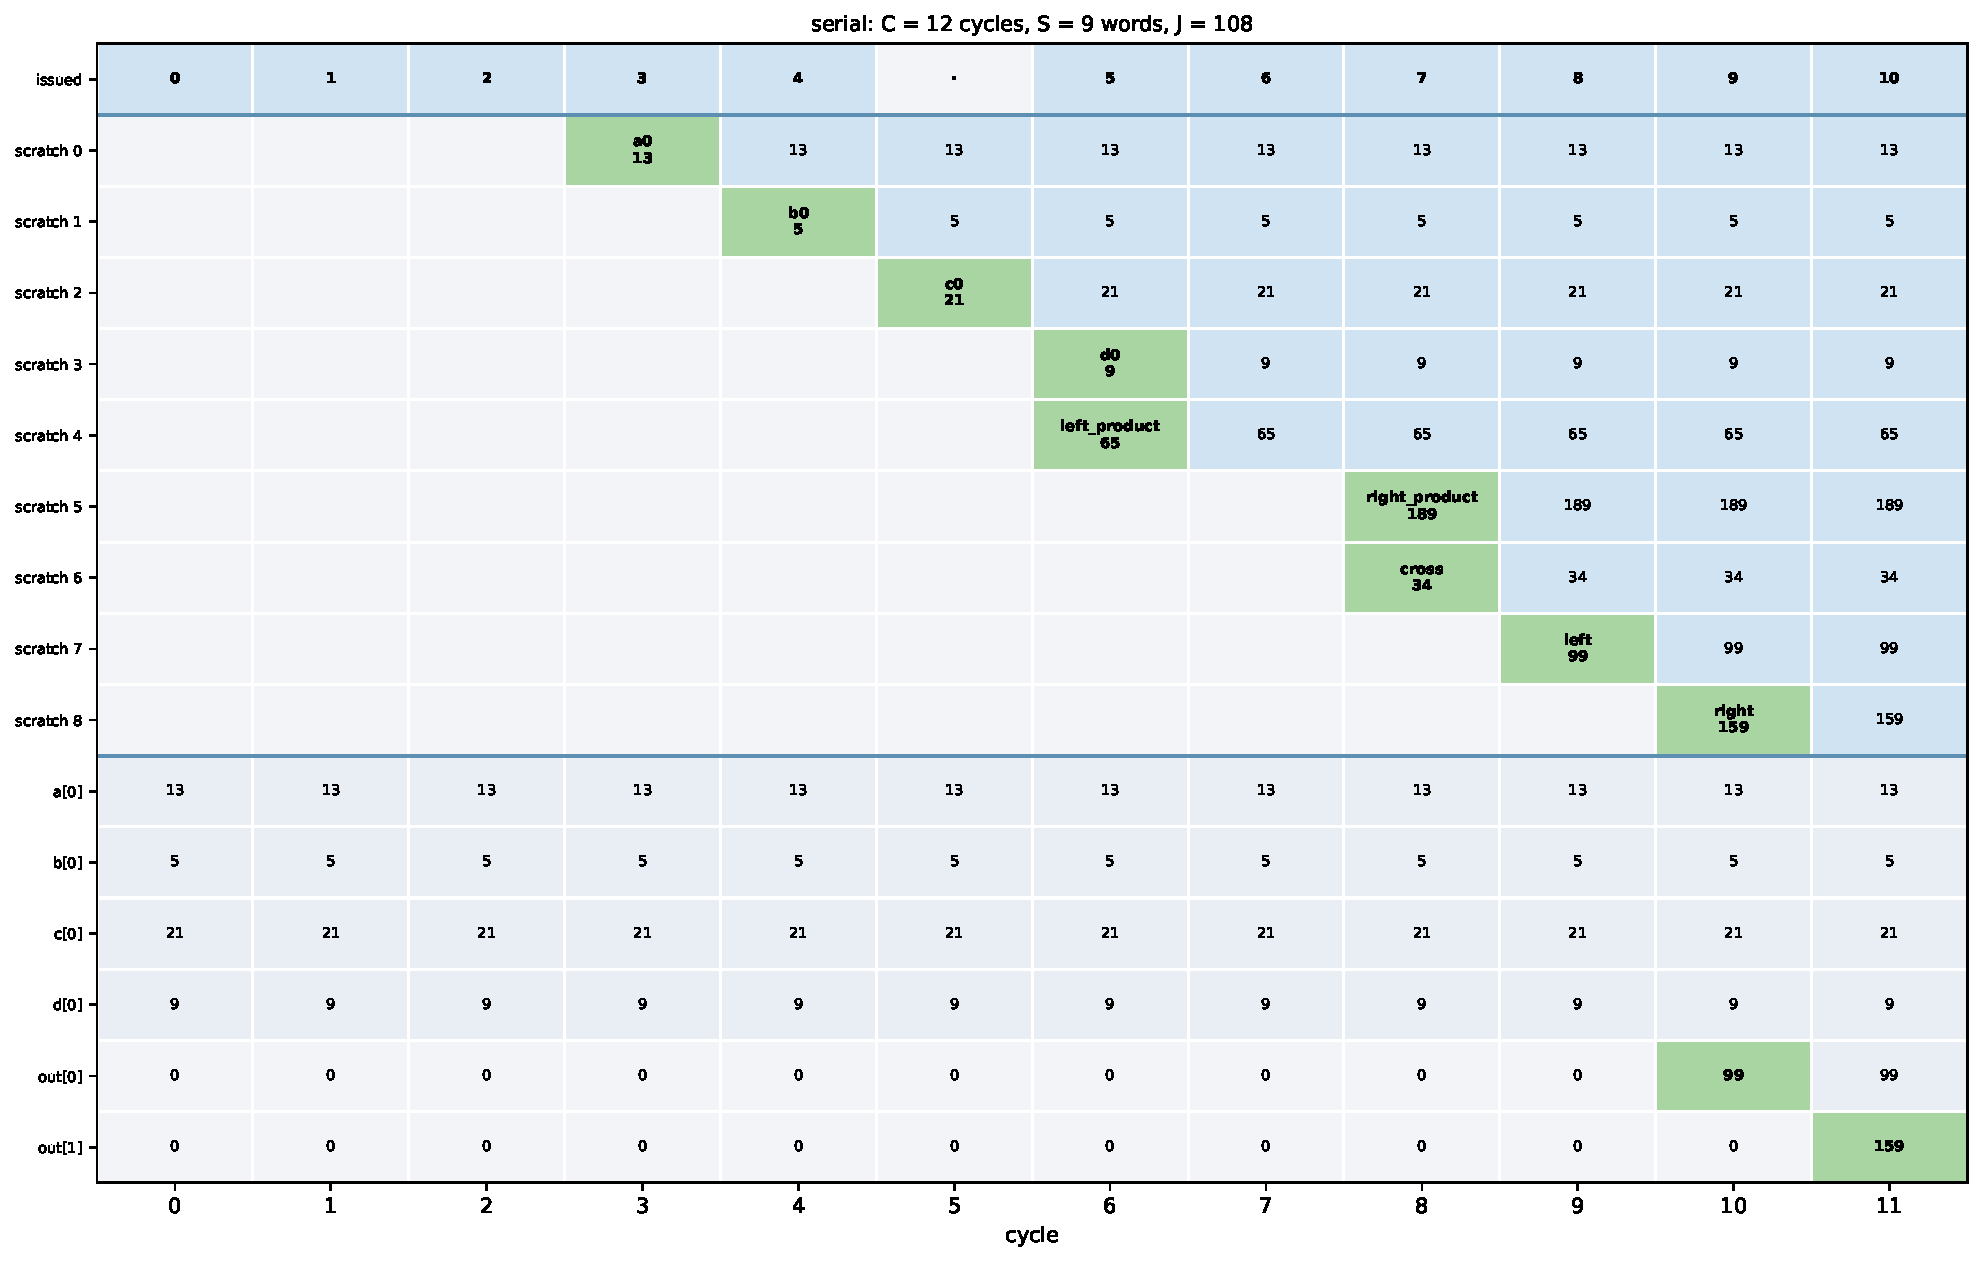
\includegraphics[width=1\linewidth]{ex_trace_serial.pdf}\par\medskip
\textbf{B}\quad classical\par
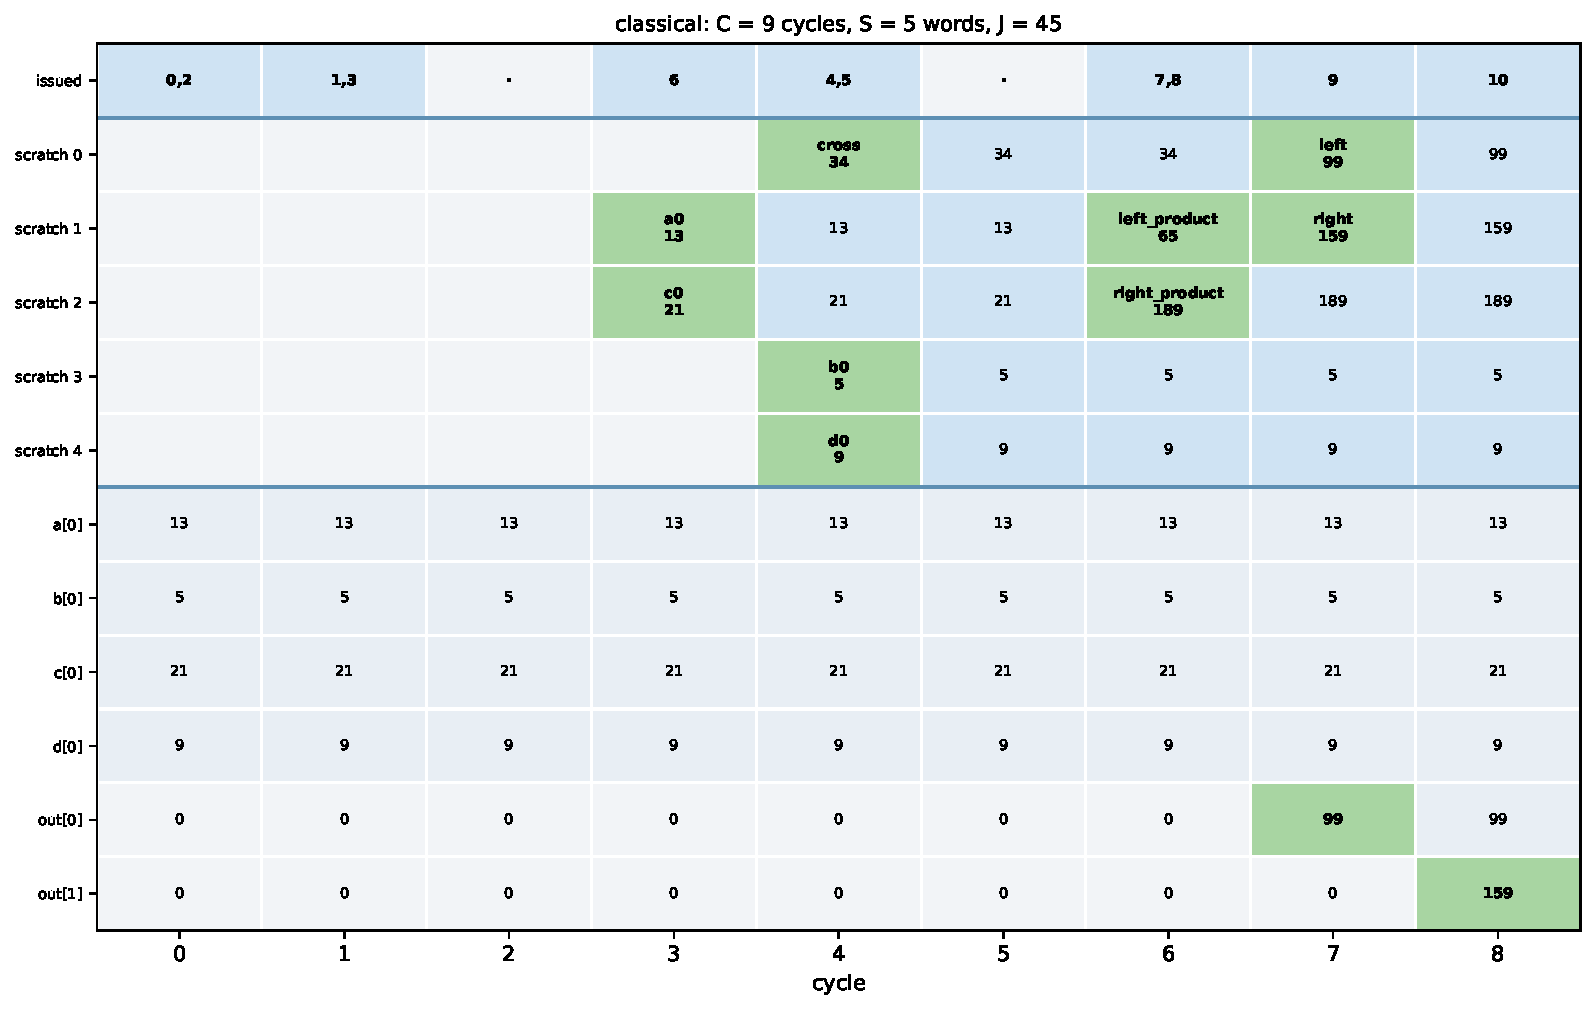
\includegraphics[width=1\linewidth]{ex_trace_classical.pdf}
\caption{\textbf{How a compiler's output runs, cycle by cycle}, on
\texttt{02\_scalar\_dual\_chain}. Columns are cycles. The top strip is the schedule
(operations issued); the middle band is the allocation (one row per scratch word,
with the value it holds); the bottom band is main memory. Green: a value landing
in its word, or a store reaching memory. (A)~Serial, $\V{exSerC}\times\V{exSerS}$.
(B)~Classical, $\V{exClC}\times\V{exClS}$: the loads are issued in two pairs, the
four inputs and \texttt{cross} are all alive at cycle \V{exClPeakCycle}, and the last
store waits a cycle for the store slot.}\label{fig:traces}
\end{figure}

\begin{figure}[htbp]\centering
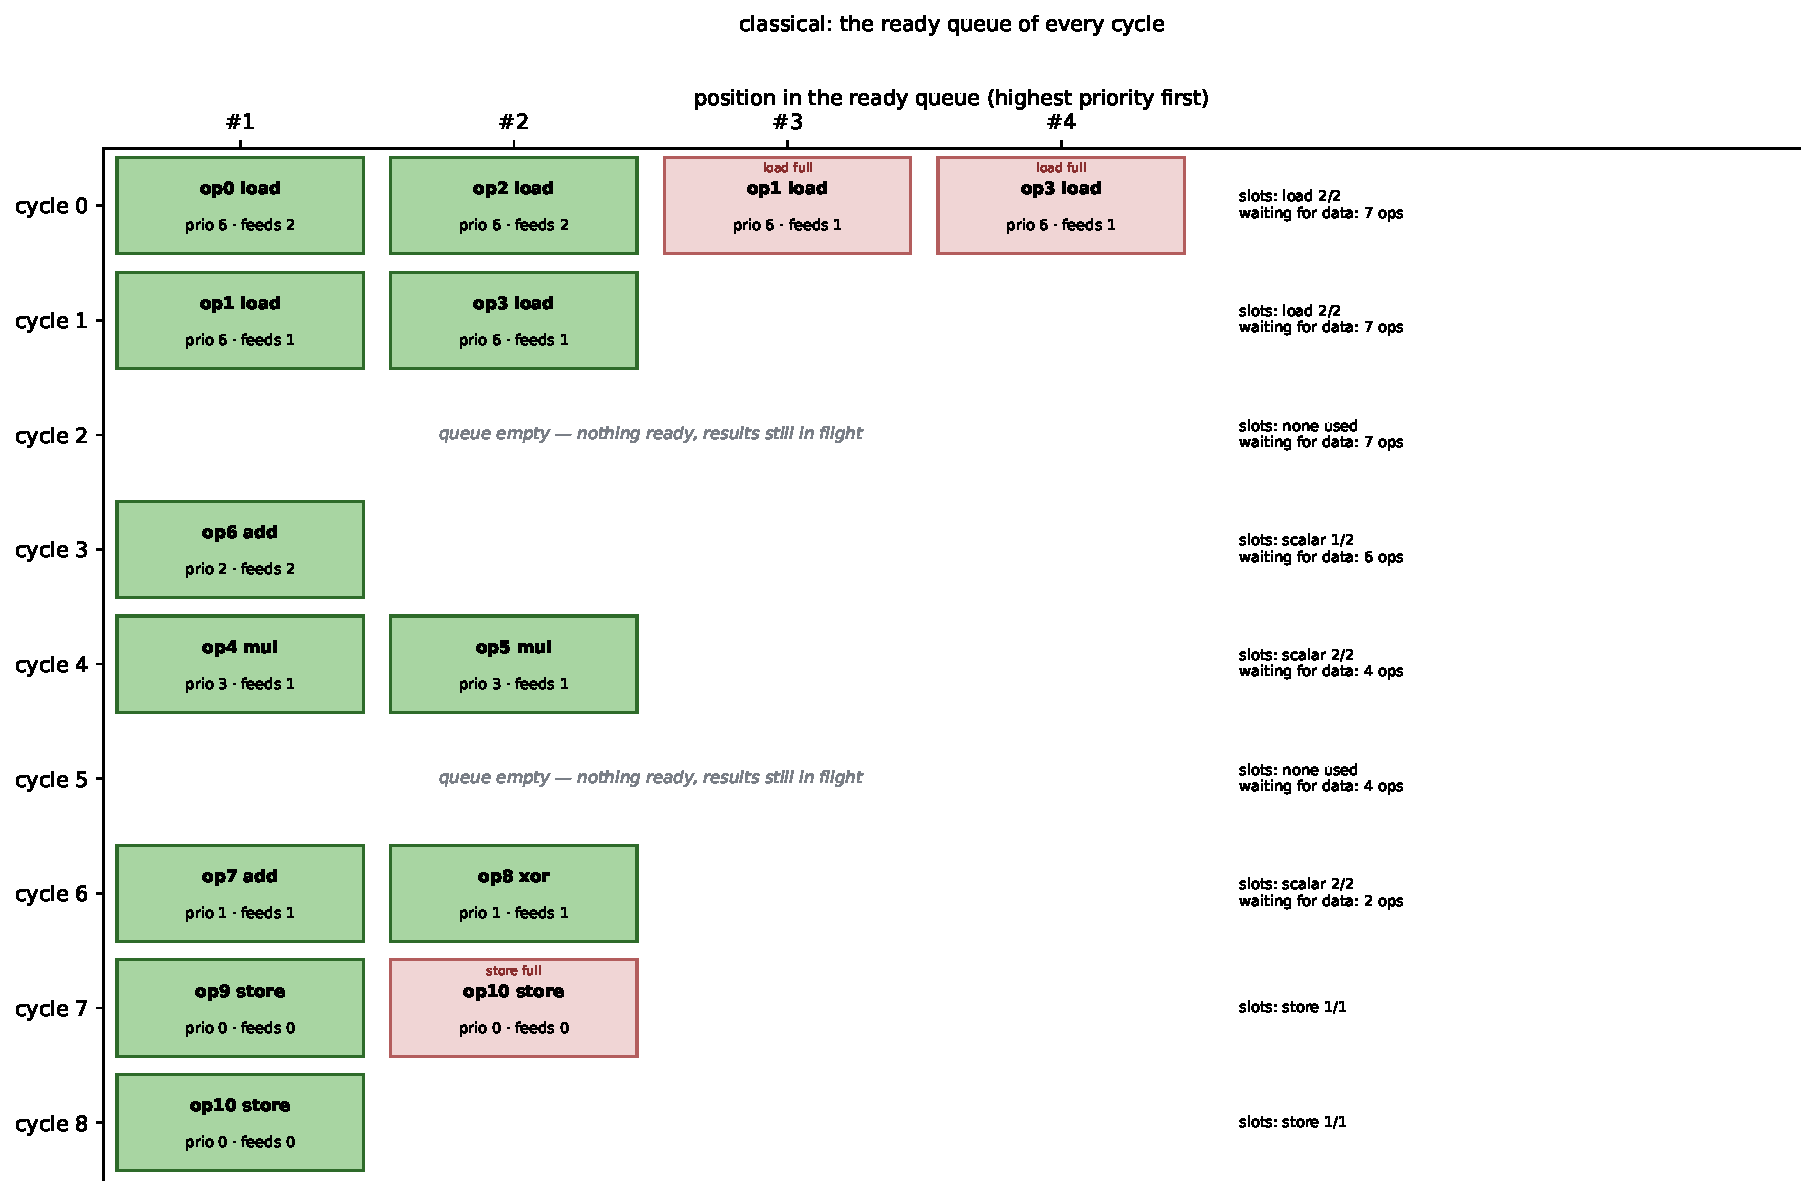
\includegraphics[width=1\linewidth]{ex_classical_queue.pdf}
\caption{\textbf{The classical list scheduler, decision by decision.} Each row is one
cycle's ready queue, sorted by priority (the longest latency chain to the end, then
fan-out). Green cards take a slot; red cards find their engine full and wait for
the next cycle. The tie among the four loads at cycle 0 is broken in favour of the
two loads that feed two operations each.}\label{fig:queue}
\end{figure}

\paragraph{Our proposal: reopen and resolve.} The compiler we propose starts from
a different question. Instead of asking ``what is the best next step?'', it asks
``which decisions are responsible for the cost I have now, and is there any way
to set them differently that lowers $J$?'' It answers that question exactly, for
small groups of decisions at a time, and repeats. We call this \emph{reopen and
resolve}; internally the final version is named C1.

The idea comes from causal deconvolution in algorithmic information
dynamics~\cite{zenil2019deconvolution,zenil2019calculus,hernandez2019aid}: an
observed outcome is explained by separating it into the contributions of the
mechanisms that produced it, and each mechanism is studied by intervening on it
while the rest is held fixed. Here the outcome is a compiled program, its cost is
$C\times S$, and the mechanisms are groups of decisions. The last operations to
issue produce $C$; the values alive at the memory peak produce $S$. Reopening one
such group while freezing everything else is an intervention, and solving it
exactly tells us whether that group can do better. The compiler does not run a
general deconvolution algorithm; it borrows this causal stance and applies it to
scheduling.

One ingredient makes this practical: the set of legal choices for a group of
decisions is kept as an exact and compact description, which can be asked
questions such as ``what is the smallest legal cycle?'' or ``is any assignment
with $J$ below the current value legal?'' without listing its members one by one.
Section~\ref{sec:steps} shows how that description is written, how a question is
asked of it, and how each answer becomes a decision. On the example it reaches
$C=\V{exOursC}$, $S=\V{exOursS}$, $J=\V{exOursJ}$, against \V{exClJ} for classical
and \V{exSerJ} for serial, and it proves that nothing better exists.

\section{Our approach, step by step}\label{sec:steps}

We follow \texttt{02\_scalar\_dual\_chain}, one of the public provided programs,
 and follow it through every step. The compiler works
by a single loop: it \emph{writes a question} about a set of options, \emph{obtains
the answer} exactly, and \emph{turns the answer into a decision}. Step~1 asks one
question per decision; Steps~2 to~5 ask questions about groups of decisions.

\paragraph{Step 1: a correct first answer, one question per decision.} Operations
are taken in program order, and for each the compiler asks: \emph{which cycles may
this operation use, given everything decided so far?} The answer is a set of cycle
numbers, and the way the set is written is what makes the question cheap.

Our compiler obeys exactly the same rules as the classical one, precedence and
engine slots; what differs is where the rules are applied. The classical compiler
applies them cycle by cycle: at each cycle it inspects every waiting operation,
checks whether its inputs have landed and a slot is free, ranks the ready ones and
issues them. Ours applies them once, when it writes the question. Before asking
about an operation it computes the earliest cycle at which its inputs have landed
(for operation 4, \texttt{left\_product}, that is cycle 3: its inputs \texttt{a0} and
\texttt{b0} are loaded at cycle 0 with latency 3), and this becomes the lower end
of the window. Cycles whose engine is already full are then removed. The set that
remains contains legal cycles only, so its smallest member is both legal and as
early as possible. Step~1 still decides one operation at a time and never revisits
an answer; each answer becomes a constraint on the questions that follow. Treating
decisions jointly is the work of Steps~2 to~5.

\emph{The binary format} has three ingredients, shown on the example in
Table~\ref{tab:codes} and Figure~\ref{fig:cube}.

\smallskip\noindent\textit{(a) Cycle numbers as bits, and the horizon.} Every cycle
number is written in binary. How many bits are needed depends on the latest cycle a
schedule could ever require. Issuing each operation only after the previous one has
completely finished is always legal, so no schedule needs more cycles than the sum
of all latencies. For the example, that sum is the sum of the all latencies for the all
operations, $\V{exLatSum}=\V{exHorizon}$, which here we call the
\emph{horizon}: no operation ever needs a cycle beyond \V{exHorizonLast}. Five bits
name the 32 cycles 0 to \V{exCodeMax}, so \V{exTimeBits} bits suffice. The same
reasoning closes each operation's own window: it ends at the sum of the latencies of
the operations before it, which is why the four loads have windows ending at 0, 3,
\V{exQhi} and \V{exWinD} (Table~\ref{tab:step1}). We write the bits lowest first, as
the implementation does: the first character is $x_0$, of weight 1, and the last is
$x_4$, of weight 16. Cycle \V{exQhi} is therefore \texttt{01100} ($2+4$) .

\smallskip\noindent\textit{(b) Cubes.} A \emph{cube} is a bit pattern in which some
positions are fixed, to 0 or 1, and the others, marked \texttt{*}, are free. It
stands for every number obtained by filling the free positions in all possible
ways, so a pattern with $k$ free positions contains exactly $2^k$ numbers. The name
comes from Boolean algebra and logic minimisation: the $2^5$ five-bit strings are
the corners of a five-dimensional cube, a pattern with no free position is one
corner, and a pattern with $k$ free positions is a $k$-dimensional face of it, a
sub-cube. Thus \texttt{00000} is the single cycle 0, and \texttt{**000} is a square
face holding cycles 0, 1, 2 and 3. The implementation stores a cube as two integers,
an \emph{anchor} (the values of the fixed bits) and a \emph{mask} of the free
positions (Figure~\ref{fig:cube}). Setting every free bit to 0 gives the anchor, so
\emph{the smallest member of a cube is its anchor}, read without listing anything.

\smallskip\noindent\textit{(c) Covers.} A single cube can only describe an aligned
block whose size is a power of two, such as $\{0, 1, 2, 3\}$ or $\{4, 5\}$. An arbitrary
range of cycles is therefore written as a union of disjoint cubes, a \emph{cover}.
The \V{exQlen} cycles from 0 to \V{exQhi} are
$\{0, 1, 2, 3\}\cup\{4, 5\}\cup\{\V{exQhi}\}$, that is \texttt{**000}, \texttt{*0100} and
\texttt{01100}, in the same way that $\V{exQlen}=4+2+1$. The number of cubes grows
with the number of bits, not with the length of the range: any range of $n$-bit
numbers needs at most about $2n$ cubes, and no question of the example needs more
than \V{exMaxCover}. Removing cycles and intersecting ranges are operations between
cubes, and the smallest member of a cover is its smallest anchor.

\begin{table}[htbp]\centering\small
\begin{tabular}{rccl}\toprule
Cycle & Bits $x_0x_1x_2x_3x_4$ & Cube in the window & Cube after the removal\\\midrule
\tableinput{generated/tab_example_codes.tex}
\bottomrule\end{tabular}
\caption{\textbf{The notation on one question} (operation 2, \texttt{load c0}). Each
cycle of the window is written with its own five binary digits, lowest first. The
window is a cover of three cubes. Removing the full cycle 0 splits the first cube
into the odd cycles, \texttt{1*000}, and the one even cycle left, \texttt{01000}; the
other two cubes are untouched. Generated from the run.}\label{tab:codes}
\end{table}

\begin{figure}[htbp]\centering
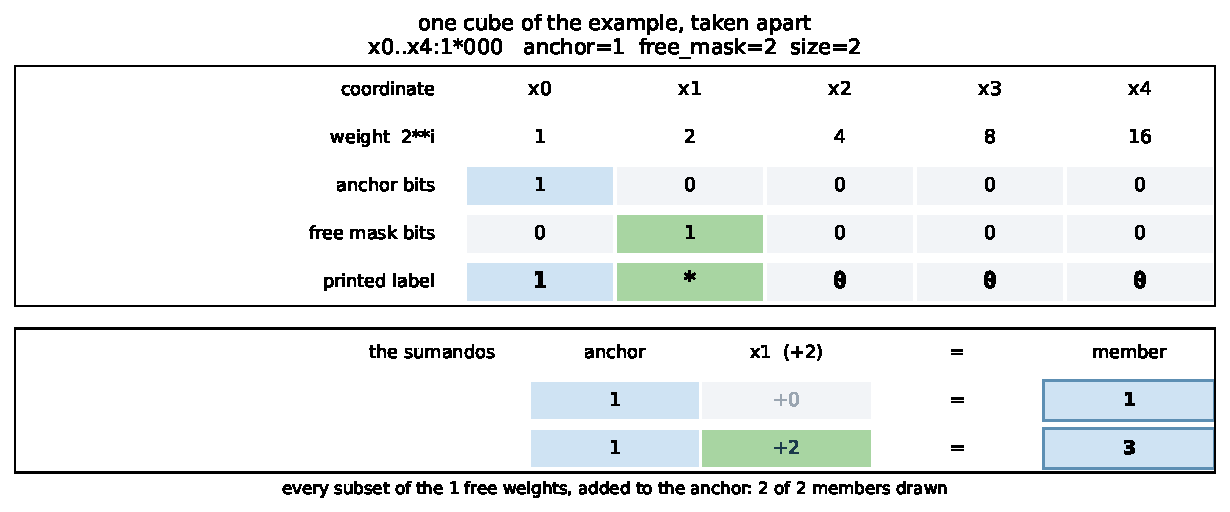
\includegraphics[width=1\linewidth]{ex_cube_anatomy.pdf}
\caption{\textbf{Anatomy of one cube}, \texttt{1*000}, from the example. Top: each
position $x_i$ has weight $2^i$; the anchor bits give the fixed part and the mask
marks the free position. Bottom: every member is the anchor plus a choice of free
weights, here $1+0$ and $1+2$, the cycles 1 and 3. The smallest member is the
anchor.}\label{fig:cube}
\end{figure}

\emph{One question, answered.} Take operation 2, the load of \texttt{c0}
(Table~\ref{tab:codes} and Figure~\ref{fig:query}). A load reads no earlier value, so
its window starts at cycle 0 and ends at \V{exQhi}: the three cubes
\texttt{\V{exQbA}}, \texttt{\V{exQbB}} and \texttt{\V{exQbC}}. Cycle 0 already holds
two loads, operations 0 and 1, and the load engine has two slots, so cycle 0 must go.
Removing it is a set difference, not a bit flip: \texttt{\V{exQbA}} minus
\texttt{00000} leaves \texttt{\V{exQaA}}, the odd cycles 1 and 3, and
\texttt{\V{exQaB}}, the cycle 2. The bits are the digits of the cycle numbers, not
one flag per cycle; the leading 1 of \texttt{\V{exQaA}} says ``odd'', not ``used''.
Nor is a cycle removed merely because something issues in it. It is removed only for
operations on the same engine, and only once that engine's slots are all taken:
cycle 1, holding one load, still accepts a second (operation 3 goes there), and a
scalar operation could still use cycle 0. The anchors of the surviving cubes are
\V{exQanchors}, so the answer is cycle 1, and the decision follows at once:
operation 2 issues at cycle 1. Every member of the surviving cover is legal, so the
decision is legal by construction, and the lost cycle has a stated cause.

\begin{figure}[htbp]\centering
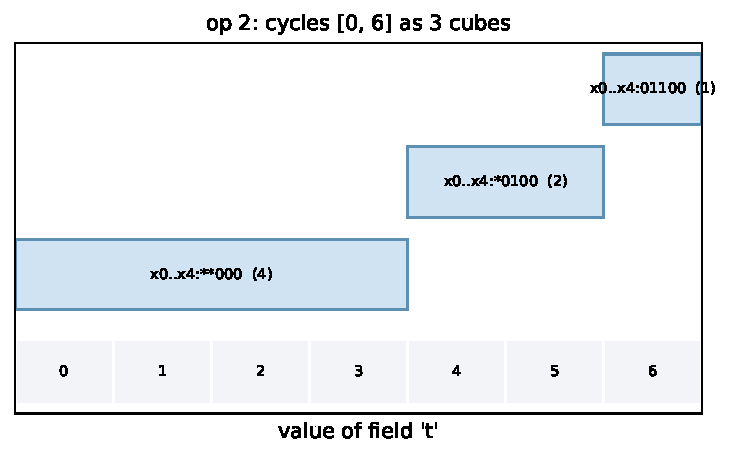
\includegraphics[width=.5\linewidth]{ex_query_before.pdf}\hfill
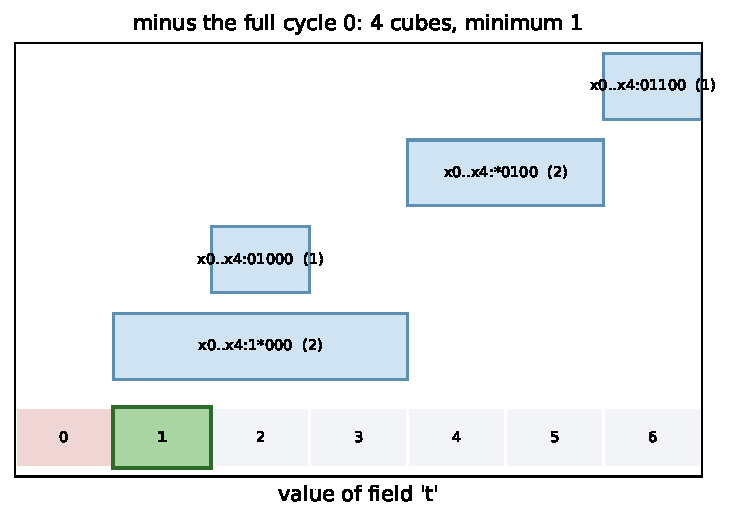
\includegraphics[width=.5\linewidth]{ex_query_after.pdf}
\caption{\textbf{One scheduling question, in the binary format.} Operation 2
(\texttt{load c0}). Left: the window of cycles it may use, written as three cubes
(bits lowest first; each bar spans the cycles its cube contains). Right: the full
cycle 0 (red) removed; the cover now has four cubes and its smallest member, cycle 1
(green), is the decision.}\label{fig:query}
\end{figure}

The same question is asked for every operation (Table~\ref{tab:step1}, top, and
Figure~\ref{fig:step1}, top). Operations that read earlier values cannot use any
cycle before their inputs land; those cycles lie outside the window. The loads of
\texttt{a0} and \texttt{b0} take cycle 0, those of \texttt{c0} and \texttt{d0} take
cycle 1, and every other operation issues in the first cycle at which its inputs have
landed and its engine has a free slot.

Addresses are chosen by the same loop, on \V{exAddrBits} bits (the 256 words of the
scratchpad): \emph{which words may this value occupy?} The window is written as
cubes, the words held by values whose lifetimes overlap this one are subtracted,
and the lowest survivor is the decision (Table~\ref{tab:step1}, bottom, and
Figure~\ref{fig:step1}, bottom). For instance \texttt{d0} lives only in cycle 4; at
that moment \texttt{a0} holds word 0 and \texttt{c0} holds word 1, so both are
removed and \texttt{d0} takes word \V{exAchosen}. Values whose lifetimes have ended
leave their words free, which is how \texttt{left\_product} reuses word 0 once
\texttt{a0} has been read for the last time. In all, \V{exQueries} questions build
the whole first answer.

\begin{table}[htbp]\centering\small
\begin{tabular}{rlllcc}\toprule
Op & Opcode & Window & Surviving cover (bits lowest first) & Removed & Cycle\\\midrule
\tableinput{generated/tab_example_times.tex}
\bottomrule\end{tabular}\par\medskip
\begin{tabular}{lllll}\toprule
Value & Lifetime & Window & Words held by an overlapping value & Word\\\midrule
\tableinput{generated/tab_example_addresses.tex}
\bottomrule\end{tabular}
\caption{\textbf{Step 1 on the example: every question and its answer.} Top: one
scheduling question per operation. The window starts where the operation's inputs
have landed; ``removed'' lists the cycles whose engine was already full; the answer
is the smallest member of the surviving cover. Bottom: one allocation question per
value. A value's lifetime runs from the cycle its result lands to the cycle of its
last reader; words held by values alive at the same time are removed, and the answer
is the lowest word left. Generated from the run.}\label{tab:step1}
\end{table}

\begin{figure}[htbp]\centering
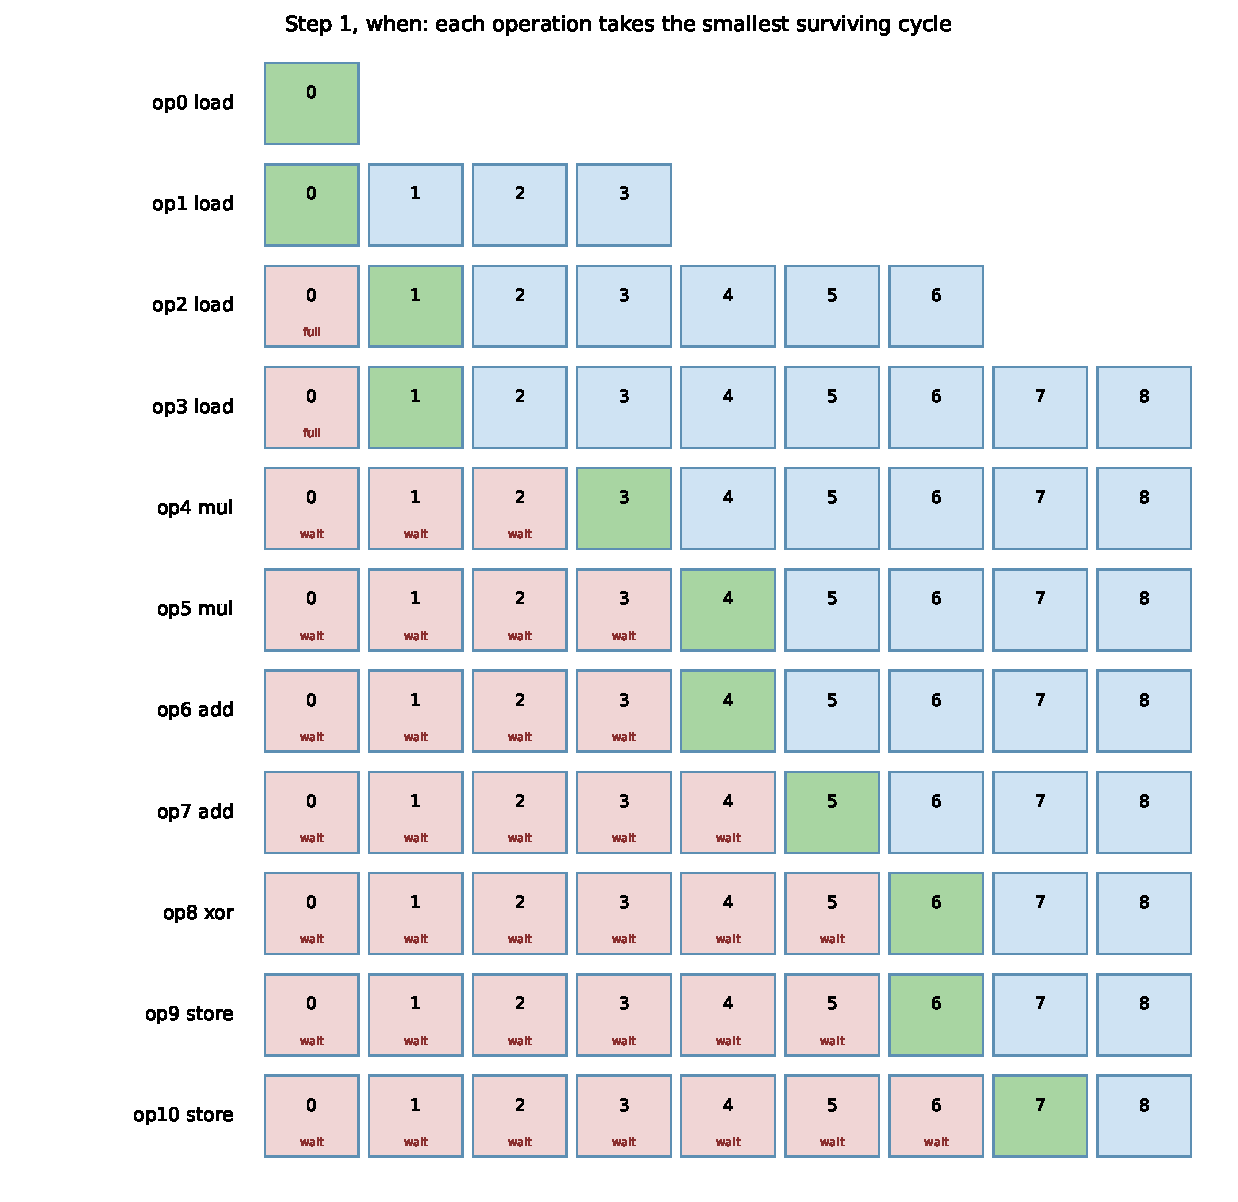
\includegraphics[width=.8\linewidth]{ex_step1_times.pdf}\par\medskip
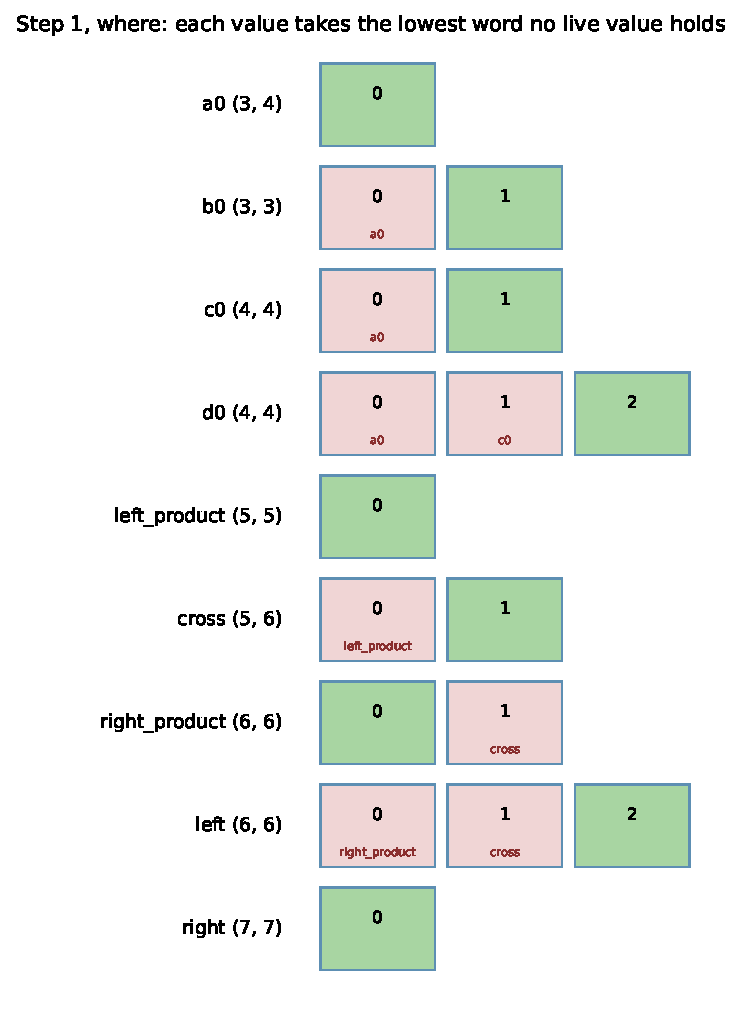
\includegraphics[width=.45\linewidth]{ex_step1_addresses.pdf}
\caption{\textbf{Step 1 as pictures.} Top: for each operation, every cycle from 0
to the end of its query window. Red cells are unavailable: \emph{wait} marks cycles
before its inputs land, which lie outside the window, and \emph{full} marks cycles
removed from the window because the engine's slots are taken; blue cells survived; green is the smallest
survivor, the decision. Bottom: the same for scratch words, one row per value with
its lifetime; a red word carries the name of the live value that holds
it.}\label{fig:step1}
\end{figure}

\emph{The result, and what it means.} Figure~\ref{fig:ours} replays the first
answer. It runs in $C=\V{exOursC}$ cycles with $S=\V{exOursS}$ words, $J=\V{exOursJ}$,
against $\V{exClC}\times\V{exClS}=\V{exClJ}$ for classical. Because the loads were
taken in pairs by chain, the left chain starts one cycle before the right one: the
two chains are staggered rather than in lockstep, their stores fall at cycles
\V{exOursStoreA} and \V{exOursStoreB} and never compete for the store slot, and at
no cycle are more than three values alive. Reading the middle band of
Figure~\ref{fig:ours} row by row shows the allocation at work: word 0 holds
\texttt{a0}, then \texttt{left\_product}, then \texttt{right\_product}, then
\texttt{right}, each arriving only after the previous tenant's last read. We should
be candid about why Step~1 does so well here: it takes operations in program order
and the earliest cycle for each, and on this program that order happens to be a good
one. It is not always so; on the program of Section~\ref{sec:worked}, Step~1 alone
is worse than classical. That is why the compiler does not stop here.

\begin{figure}[htbp]\centering
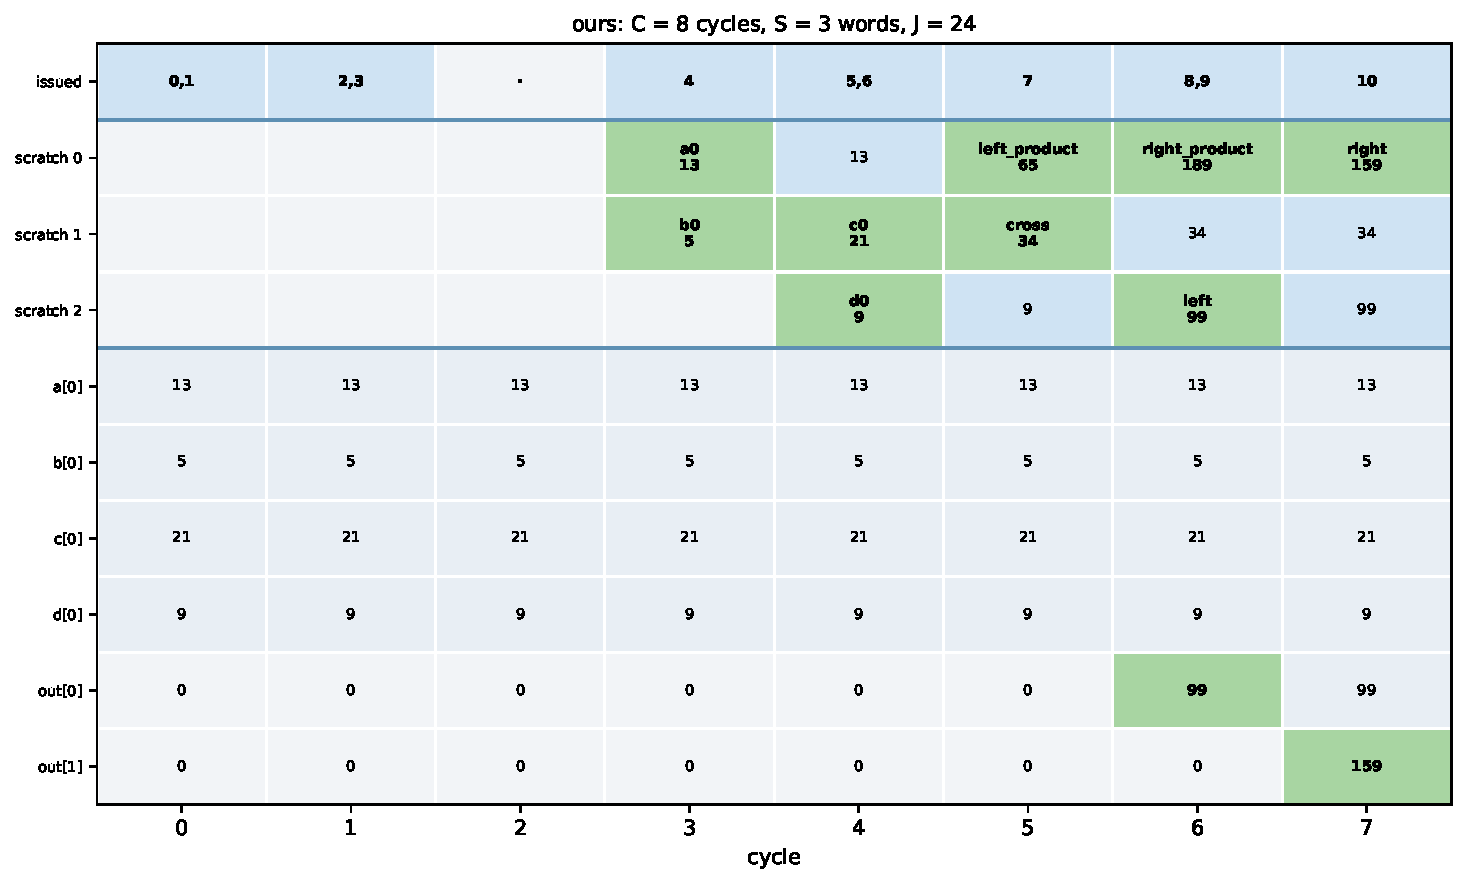
\includegraphics[width=1\linewidth]{ex_trace_ours.pdf}
\caption{\textbf{Our compiler's output on the example}, in the same picture as
Figure~\ref{fig:traces}: $\V{exOursC}\times\V{exOursS}$. The chains are staggered by
one cycle, the stores never collide, and three words are reused by all
\V{exValues} values.}\label{fig:ours}
\end{figure}

\paragraph{Step 2: find the decisions that cause the cost.} The compiler builds a
\emph{catalogue} of groups of related operations, called windows, each allowed to
move its issue cycles within a radius while everything outside the window stays
fixed. The catalogue deliberately targets the causes of cost: the $k$ latest
operations, which determine $C$; the $k$ operations around the memory peak, which
determine $S$; contiguous blocks; small groups of four; and the whole program when
it is small. This is large neighbourhood search~\cite{shaw1998}: move several
related decisions together, because useful improvements rarely come one decision
at a time. Each window becomes one question: \emph{if only these decisions may
change, is there any legal answer with a smaller $J$?} On the example the catalogue
holds \V{exCatalogue} such questions (Figure~\ref{fig:reopen}, left), from windows of
a single operation up to the whole program.

\paragraph{Step 3: say exactly what ``better'' must look like.} With the rest of
the program fixed, a window's answer cannot use fewer than $L_C$ cycles or fewer
than $L_S$ words. If the current cost is $J_0$, a strict improvement must satisfy
$C\times S\le J_0-1$, and therefore
\begin{equation}\label{eq:box}
C\le\Bigl\lfloor\frac{J_0-1}{L_S}\Bigr\rfloor ,\qquad
S\le\Bigl\lfloor\frac{J_0-1}{L_C}\Bigr\rfloor .
\end{equation}
Every improvement lies inside this box, so the search is confined to it without
losing any. If a bound falls below its minimum, the window provably holds no
improvement and is answered without searching. This is how the objective of
Equation~\eqref{eq:j} enters the search directly: the compiler never asks for
fewer cycles or fewer words in isolation, only for a smaller product.

On the example $J_0=\V{exOursJ}$. For the \V{exBoxPolicy} window the fixed part of the
program already forces $L_C=\V{exBoxLC}$ and $L_S=\V{exBoxLS}$, so the box is
$C\le\V{exBoxCcap}$ and $S\le\V{exBoxScap}$; both bounds lie below their minimums,
the box is empty, and the question is answered by arithmetic alone. \V{exBoxClosed}
of the \V{exCatalogue} questions end this way. For the whole-program window the
minimums are $L_C=\V{exWholeLC}$ and $L_S=\V{exWholeLS}$, and the box is $C\le
\V{exWholeCcap}$ (the horizon) and $S\le\V{exWholeScap}$: any improvement must use at
most \V{exWholeScap} words and fit under the curve $C\times S=\V{exOursJ}$
(Figure~\ref{fig:reopen}, right).

\paragraph{Step 4: delete impossible options, each with a reason.} Before
searching, the compiler removes choices that cannot be part of any legal answer.
If $v$ reads the result of $u$ and $u$ has latency $\ell$, then $v$ cannot issue
before $u$'s earliest cycle plus $\ell$, and $u$ cannot issue after $v$'s latest
cycle minus $\ell$. If an engine's slots in a cycle are all taken, that cycle is
removed from every other operation on that engine. Every removal records a short
\emph{certificate} that anyone holding the program can check in one line, in the
spirit of explained propagation in constraint solvers~\cite{ohrimenko2009}. These
are the causes in the causal reading: not only ``this option is gone'', but ``this
option is gone because $v$ reads $u$ with latency $\ell$''. On the example,
\V{exRootClosed} further questions are closed here, before a single search node:
at the root, propagation together with the lower bound on $J$ already rules out
every combination inside the box, which proves the window holds no improvement.

\paragraph{Step 5: search exactly, keep the first validated improvement, repeat.}
What remains is searched exactly, depth first, abandoning any branch whose best
possible $J$ is no better than the current one. A controller keeps \V{resident}
windows open at once and gives each a short turn of at most \V{sliceMs}\,ms, so no
single hard window can consume the budget. The first window to find a strict
improvement wins: its answer is checked by the challenge's own validator, becomes
the new current answer, and a new round starts from it. The submitted compiler stops
after \V{bB}\,s or when a whole round finds nothing. This is the combinatorial view of
scheduling and allocation of Casta\~neda Lozano and colleagues~\cite{castaneda2019},
applied to small, well-chosen neighbourhoods rather than to the whole program at once.

On the example only \V{exSearched} questions survive to the search: the window of
the 16 latest operations and the whole-program window, which on a program of
\V{exOps} operations release the same operations with different radii. Both are searched to the end, in \V{exNodes} nodes in total
(\V{exWholeNodes} for the whole-program window), and neither contains a strict
improvement. The round finishes having found nothing, so the compiler stops after
\V{exEpochs} round, long before its budget, and returns the first answer unchanged,
together with \V{exCerts} certificates that justify every option it discarded. This
agrees with an independent check that shares nothing with the search: enumerating
all \V{exOptSchedules} legal schedules of at most \V{exOptCmax} cycles (the only
ones that could reach $J\le\V{exOptJm}$, because every two-operand operation needs
two words at once, so $S\ge2$) finds none below \V{exOursJ}. On this program our
answer is optimal, and the classical one is \V{exRatioCl} times the optimum.

\begin{figure}[htbp]\centering
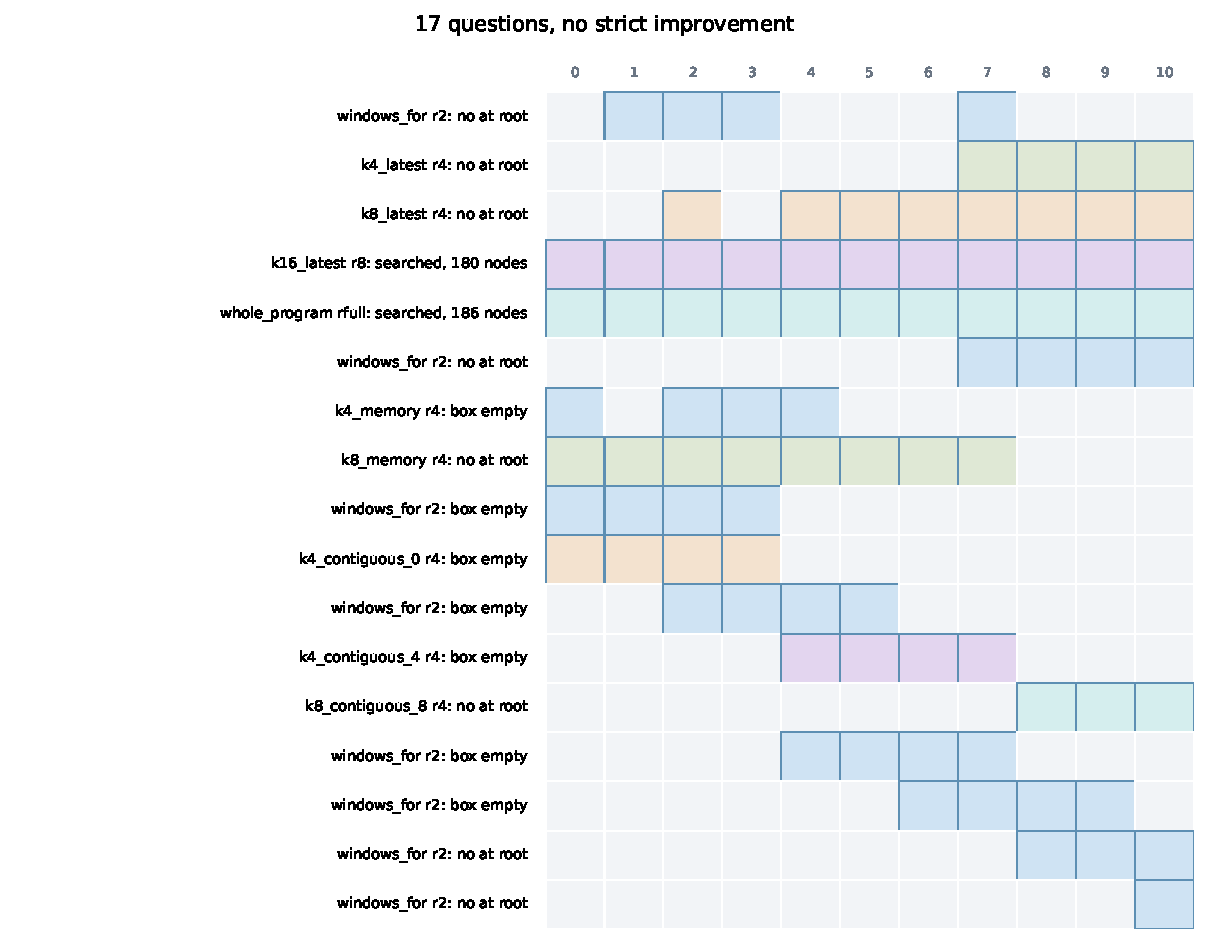
\includegraphics[width=1\linewidth]{ex_catalogue.pdf}\hfill
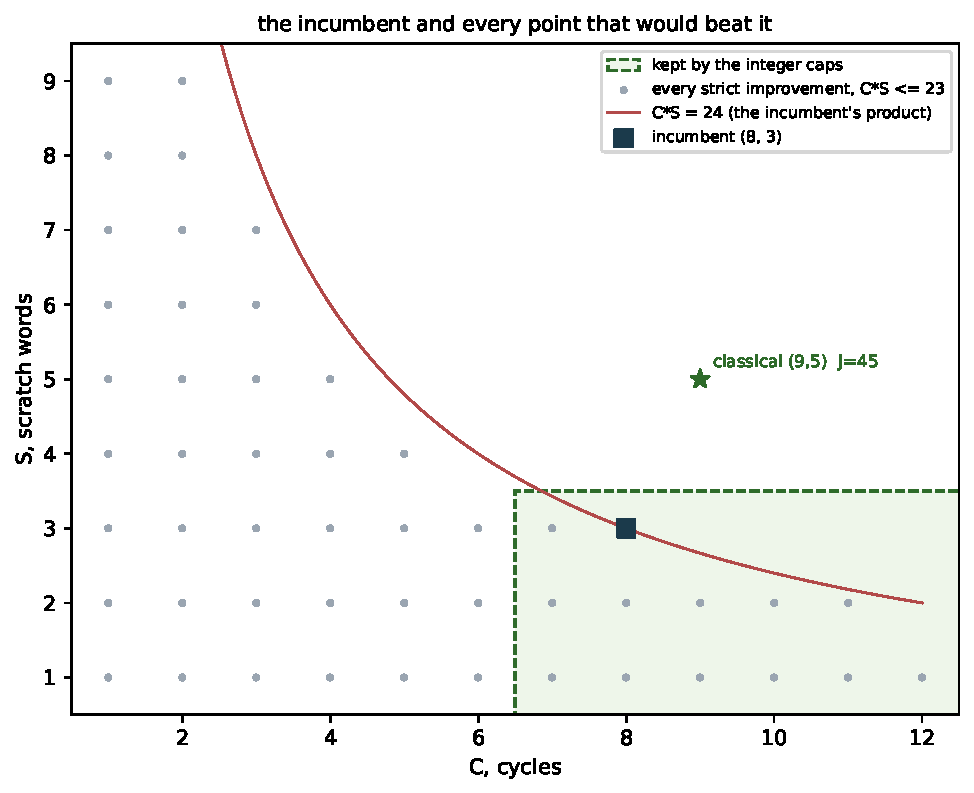
\includegraphics[width=.6\linewidth]{ex_plane.pdf}
\caption{\textbf{Reopen and resolve on the example.} Left: the \V{exCatalogue}
questions of the round, one row per window; a filled cell is an operation that
question may move, and the label gives its verdict (box empty, closed at the root
by propagation, or searched to the end). Right: the $(C,S)$ plane. Grey dots are
all points with $C\times S\le\V{exOptJm}$, that is every strict improvement; the curve
is $C\times S=\V{exOursJ}$; the dashed box is the whole-program question's region. The
search proves that no legal compilation lies in it.}\label{fig:reopen}
\end{figure}

\paragraph{Why this came out better.} The example isolates the three differences.
First, the classical scheduler decides by a local, time-only rule: the tie among the
loads was broken by fan-out, and that one choice put both chains in lockstep, which
cost a cycle at the store slot and two words at the memory peak. Steps~2 to~5 judge
every question by $J$ itself, so a schedule that saves memory is never discarded for
failing to save time. Second, each of our decisions is the exact answer to a
question about a set of legal options, written compactly as cubes, so no legal option
inside a question is overlooked and nothing illegal is ever produced; every removal
has a stated cause.
Third, our compiler knows when to stop looking: here, a single round of \V{exNodes}
nodes proves that no window, including the whole program, can do better, which is a
guarantee the classical compiler cannot give. On this program Step~1 already found
the optimum and Steps~2 to~5 certified it; on the program of
Section~\ref{sec:worked} it is Steps~2 to~5 that turn a first answer worse than
classical into one that beats it.

\paragraph{An engineering refinement.} A search node differs from its parent by a
single decision, yet a naive implementation re-checks every constraint at every
node. The final version keeps, at each node, the facts its parent had already
derived and re-examines only the constraints that the new decision can reach.
Measured on \V{tPrograms} fresh programs at identical search work
(\V{tNodes} nodes), it makes exactly the same decisions as the version without the
refinement in \V{tParityPairs} of \V{tParityPairs} paired runs, and its compile call
takes \V{tCost} of the time (\V{lvThree}\% interval \ci{\V{tCostLo}}{\V{tCostHi}}). Because
it is faster, it explores more within the same wall-clock budget; at \V{bB}\,s its
geometric-mean $J$ is \V{tQual} of the unrefined version's (interval
\ci{\V{tQualLo}}{\V{tQualHi}}).

\section{A worked example: \texttt{05\_mixed\_broadcast}}\label{sec:worked}

We now follow one public program from the challenge repository through every
compiler. Figure~\ref{fig:program} shows it: \V{weOps} operations, three loads, two
\texttt{splat}s that copy a scalar into all eight lanes of a vector, a vector
multiply, a vector add and a vector store. Its difficulty is easy to see. The
vector load is slow, several eight-word vectors are alive together, and the order
in which the vectors are created decides how much scratch they need.

\begin{figure}[htbp]\centering
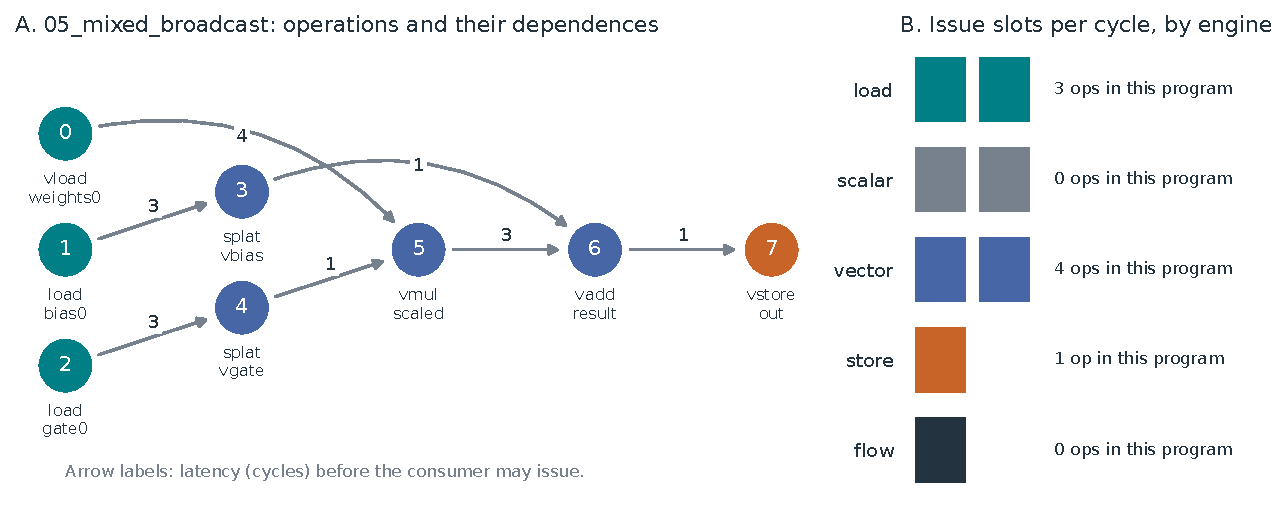
\includegraphics[width=\linewidth]{we_program.pdf}
\caption{\textbf{The worked example.} (A)~Operations and their dependences; each
arrow is labelled with the latency that must pass before the consumer may issue.
(B)~Issue slots per cycle for each engine.}\label{fig:program}
\end{figure}

\paragraph{Serial.} One operation per cycle and a fresh address for everything:
$C=\V{weSerialC}$, $S=\V{weSerialS}$, $J=\V{weSerialJ}$. This is the yardstick.

\paragraph{Classical.} The list scheduler issues the three loads as early as the
two load slots allow, starts the vector work as soon as inputs arrive, and first
fit reuses words as soon as values die: $C=\V{weClassicalC}$, $S=\V{weClassicalS}$,
$J=\V{weClassicalJ}$. It is a big improvement over serial, and on this program the
greedy choices are good.

\paragraph{Our Step 1.} The first answer takes, for every operation, the earliest
legal cycle; for instance operation~\V{weQTop} could issue anywhere in cycles
\V{weQTlo} to \V{weQThi}, cycle \V{weQTlo} is already full on the load engine, and so
it takes cycle \V{weQTchosen}. It then gives each value the lowest legal address.
The result is $C=\V{weDirectphase1C}$, $S=\V{weDirectphase1S}$,
$J=\V{weDirectphase1J}$: legal, but \emph{worse than classical}. Issuing every
vector as early as possible keeps two eight-word vectors alive together, and that
costs memory. A compiler that stops here loses to the classical one on this program.

\paragraph{Our Steps 2 to 5.} The compiler now reopens. It builds a catalogue of
\V{weCatalogue} windows (Figure~\ref{fig:pipeline}B). For the window that releases
the latest operations, the fixed part implies at least \V{weCapLC} cycles and
\V{weCapLS} words, and the box of Equation~\eqref{eq:box}, with the cycle bound also
limited by the search horizon, becomes $C\le\V{weCapCcap}$ and $S\le\V{weCapScap}$.
Inside it, the declared combinations of issue cycles number \V{weCombDeclared};
propagation with \V{weRootCerts} certificates reduces them to \V{weCombRoot} before
any search begins. The search then walks the path shown in
Figure~\ref{fig:pipeline}C:
\begin{itemize}
\item the first round, through the window of the latest operations, keeps the same
number of cycles and cuts the footprint: $\V{weStepAC}\times\V{weStepAS}$;
\item the second round, through the same window, saves a cycle:
$\V{weStepBC}\times\V{weStepBS}$, level with classical;
\item the third round, through a small window of four operations that had nothing to
offer at the start, saves one more word: $\V{weStepCC}\times\V{weStepCS}$.
\end{itemize}
The final answer, $C=\V{weC1C}$, $S=\V{weC1S}$, $J=\V{weC1J}$, beats the classical
compiler. It took \V{weEpochs} rounds and \V{weNodes} search nodes, and every
intermediate answer was validated by the challenge's checker. Notice the pattern:
a large window opened the way and a small one finished it. Neither kind of move
alone reaches this answer.

\begin{figure}[htbp]\centering
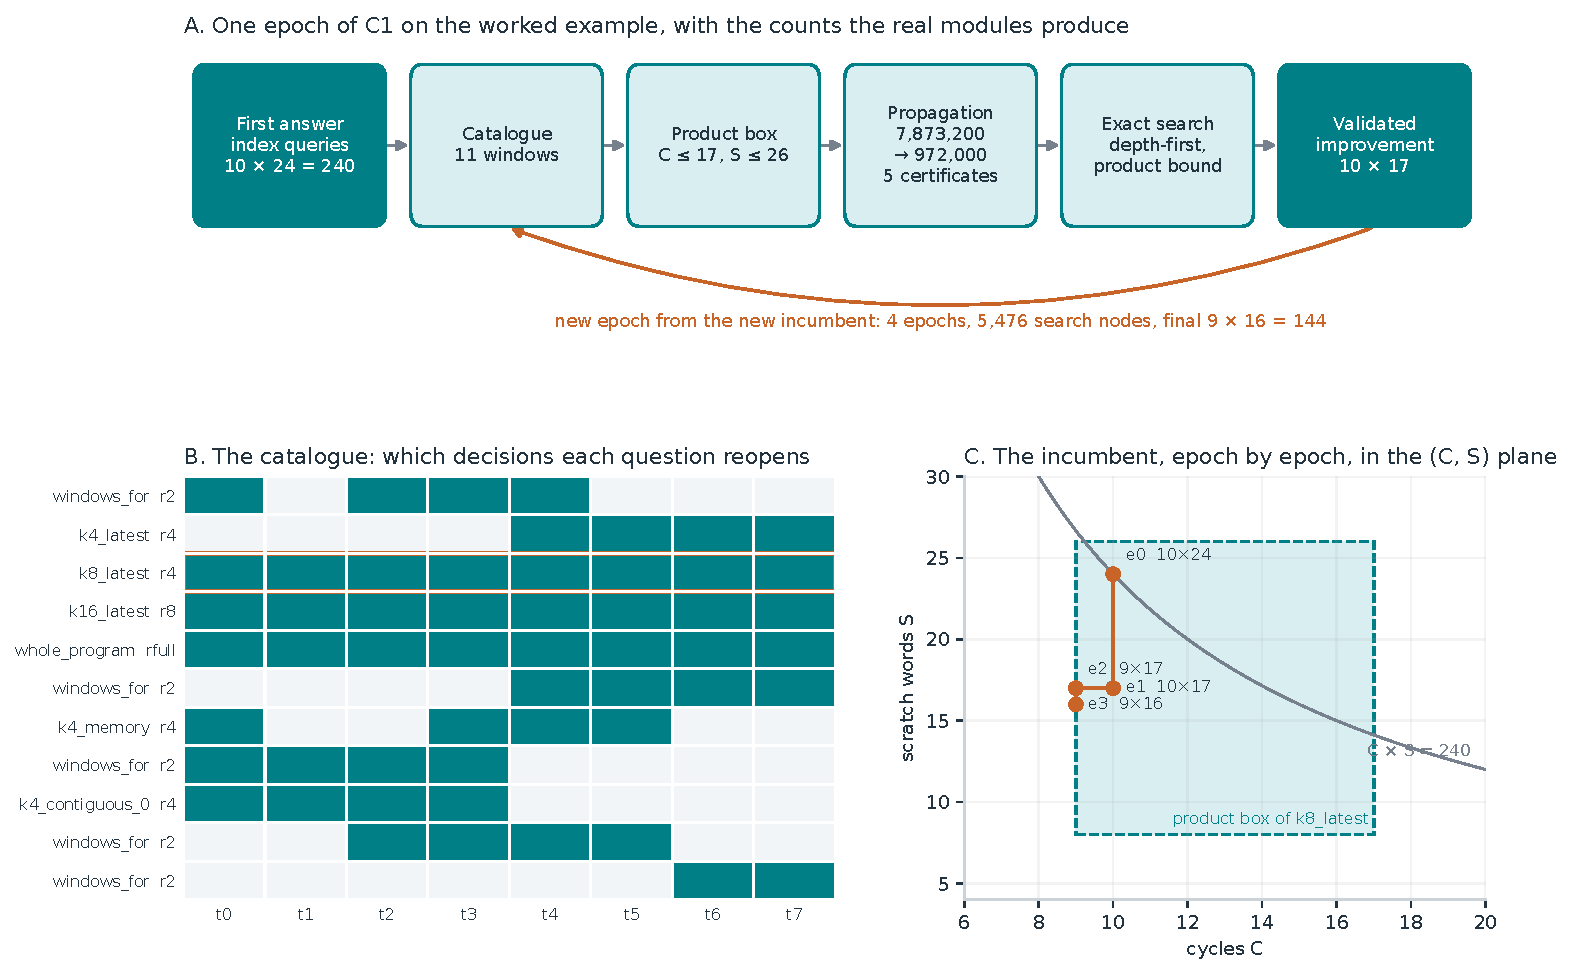
\includegraphics[width=\linewidth]{we_pipeline.pdf}
\caption{\textbf{Reopen and resolve on the worked example.} (A)~One round, with
the counts that the real compiler produces. (B)~The catalogue: each row is one
window and each filled cell an operation it may move. (C)~The current answer, round
by round, in the $(C,S)$ plane; the curve is the starting value of $J$, the shaded
region the box of Equation~\eqref{eq:box}.}\label{fig:pipeline}
\end{figure}

Figure~\ref{fig:methods} puts the schedules and memory layouts side by side. The
difference between classical and ours is visible in the lower panels. Both keep
the vectors inside two eight-word blocks; the difference lies in the scalars. The
classical layout places one scalar above the vector blocks, which raises the
footprint by one word. Ours issues the scalar loads so that each scalar lives in
words that no vector occupies at that moment, and the footprint closes exactly at
the top of the second block.

\begin{figure}[htbp]\centering
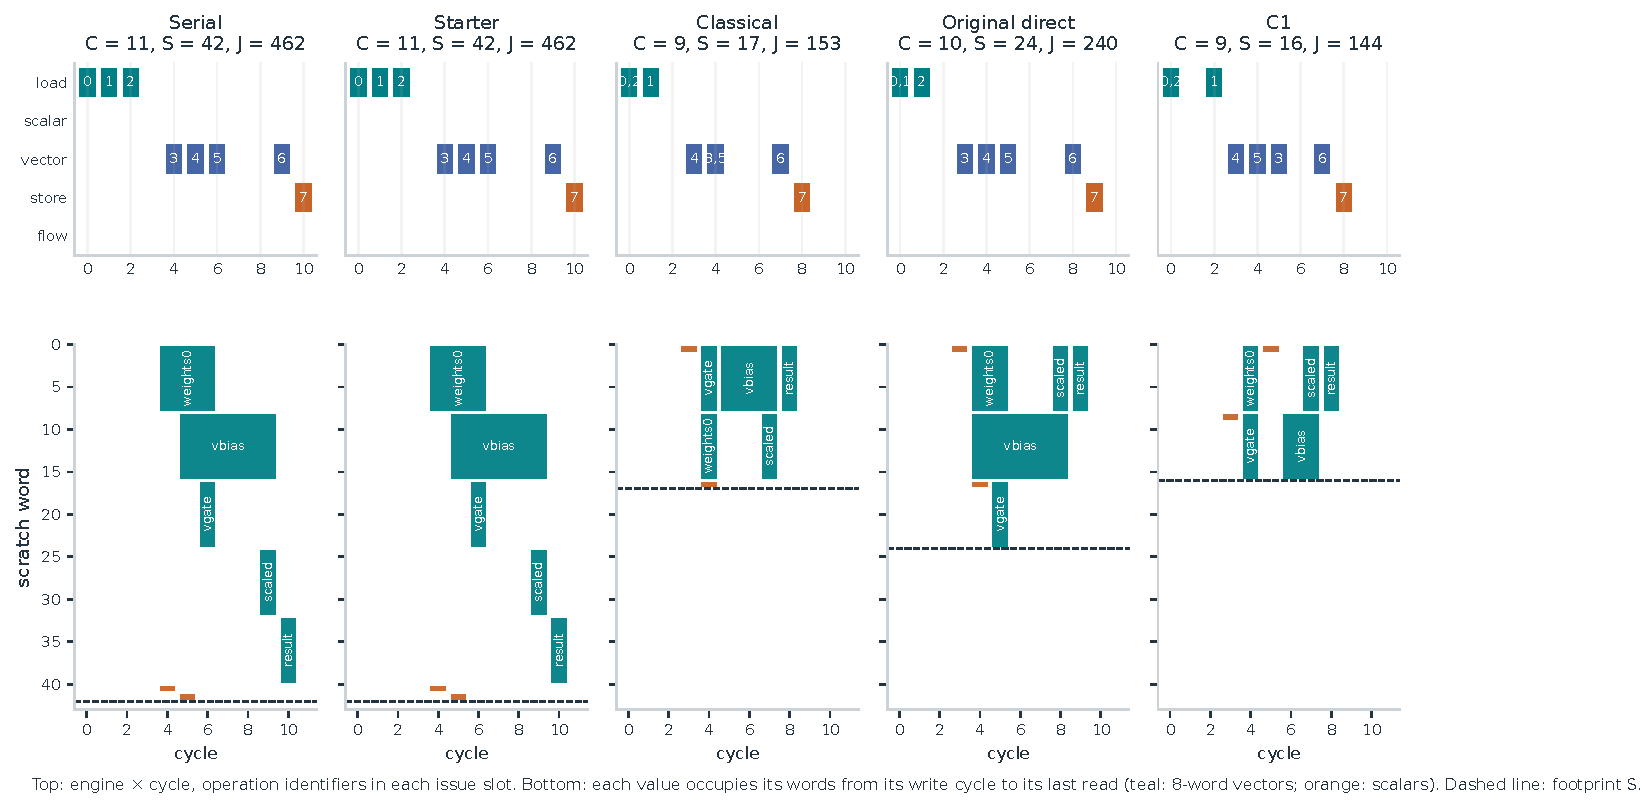
\includegraphics[width=\linewidth]{we_methods.pdf}
\caption{\textbf{Every compiler on the same program.} Top: engine by cycle, with the
operations issued in each slot. Bottom: scratch words by cycle; each value occupies
its words from its write to its last read, and the dashed line is the footprint $S$.
``Original direct'' is our Step~1 alone; ``C1'' is the full compiler. Every layout
was produced by running the compiler and checked by the challenge's validator.}
\label{fig:methods}
\end{figure}

\section{Results against the classical benchmark}\label{sec:results}

\subsection{The public programs}
Table~\ref{tab:public} gives every public program. Our compiler is better than
classical in $J$ on \V{rpBetter} programs and equal on \V{rpEqual}; it is never
worse. Its geometric-mean $J$ is \V{rpJRed}\% below classical, and its score is
\V{tPubSixC1B} against \V{rTwoPubClassical}.

\begin{table}[htbp]\centering\small
\begin{tabular}{lrrrrrr}\toprule
& \multicolumn{3}{c}{$C\times S$} & \multicolumn{3}{c}{$J$}\\
\cmidrule(lr){2-4}\cmidrule(lr){5-7}
Program & Serial & Classical & Ours & Serial & Classical & Ours\\\midrule
\tableinput{generated/tab_public.tex}
\midrule
\multicolumn{4}{l}{Cycle speedup over serial} & 1 & \V{rpCycCl} & \V{rpCycCOne}\\
\multicolumn{4}{l}{Scratch reduction over serial} & 1 & \V{rpScrCl} & \V{rpScrCOne}\\
\multicolumn{4}{l}{\textbf{Combined score} (Equation~\ref{eq:score})} & 1 & \V{rTwoPubClassical} & \textbf{\V{tPubSixC1B}}\\
\bottomrule\end{tabular}
\caption{The eight public programs. ``Ours'' is the submitted configuration, with a
\V{bB}\,s search budget; bold marks the lowest $J$ in each row. Every value was
identical in each of \V{tReps} fresh-process repetitions, and every compilation
passed the challenge's validator on all supplied cases.}\label{tab:public}
\end{table}

The split between the two halves of the score is the most instructive part of the
table. Our compiler uses fewer scratch words than classical on \V{rpScrBetter} of the
eight programs, but fewer cycles on only \V{rpCycBetter}, and more cycles on
\V{rpCycWorse}. On \texttt{vector\_axpy}, for example, it accepts one more cycle to
halve the footprint. That is not an accident; it is the objective at work. Because
the score weighs time and memory equally, one extra cycle on a program of about ten
cycles is a good trade for half the memory, and a compiler that searches the product
$C\times S$ finds such trades, where one that optimises cycles first cannot see them.

\subsection{Programs never seen during development}
The public programs were visible while we built the compiler, so they show exact
results on eight fixed programs, not an estimate of performance on unseen ones. To
test generalisation we generated fresh programs in five families (scalar, vector,
mixed, dependency-heavy and memory-aliasing) only after each version was frozen.
The direct predecessor of our final compiler, which runs the same catalogue and the
same depth-first search, was compared with the classical compiler on \V{tPrograms}
such programs with a \V{bB}\,s budget: its geometric-mean $J$ was
\V{rTwoDfsClRed}\% lower (a descriptive comparison, without an interval), with \V{rTwoDfsClW} programs better, \V{rTwoDfsClT} equal and
\V{rTwoDfsClL} worse. An earlier version with the same catalogue, on another fresh
cohort of \V{tPrograms} programs, was \V{rOneClRed}\% lower (\V{lvOne}\% interval \V{rOneClLo}\% to
\V{rOneClHi}\%), with \V{rOneClwins} better, \V{rOneClties} equal and \V{rOneCllosses}
worse. The final compiler adds only the engineering refinement of
Section~\ref{sec:steps}, which makes the same decisions at equal work; it was not
itself re-measured against classical on a fresh cohort, and we do not multiply
results across rounds.

\subsection{What it costs}
Compile time is the price. The classical compiler compiles a public program in a
median of \V{rpClCallMed}\,ms. Ours is designed to use its budget: its median compile
call is \V{rpC1CallMed}\,ms, and the slowest of its \V{rpC1Runs} public runs took
\V{rpC1ProcMax}\,s as a whole process, including interpreter start. On the fresh
cohort of round one, the search took \V{rOneClTime} times the classical compile time.
The grader allows 20\,s per program, so both are far inside the limit; the
difference is that the classical compiler leaves almost all of that allowance
unused, while ours converts a small part of it into better output.

\section{Why this approach}\label{sec:why}

\paragraph{It optimises what is scored.} Every question the search asks is framed
in terms of $J=C\times S$, the quantity the score rewards. Trades between time and
memory are therefore found, not forbidden.

\paragraph{It explains itself.} Every option the compiler rejects carries a
certificate that states its cause, and every accepted change is validated by the
challenge's own checker before it is kept. One can ask of any output why a cycle
was not used or why a value moved, and receive a concrete answer.

\paragraph{It proves when to stop looking.} When a window's box is empty, or its
exact search finishes without an improvement, that window provably has nothing
better to offer given the rest of the program. Effort goes to windows that can
still pay.

\paragraph{It is anytime and budget-aware.} A correct answer exists after Step~1,
and every later round only improves it, so the compiler can be stopped at any moment
with a valid schedule. A larger budget buys more quality; a smaller one still
returns something good. On the public programs even a budget of \V{bA}\,s scores
\V{tPubSixC1A}.

\paragraph{It generalises by construction.} Nothing refers to program names,
operation identifiers or constants; the catalogue is derived from the structure of
each program. For a company that compiles whole models into single kernels, where a
scheduler must place work in time and memory together, a search that can reopen
any group of decisions and explain each change seems to us the right foundation to
build on.

\section{Correctness and reproducibility}\label{sec:correct}

The submitted compiler is a single standard-library Python file that exposes
\texttt{compile\_program} and follows the challenge's command-line contract. It
passes the unchanged public test suite. Beyond the public programs it was run on a
corpus of \V{tAccPrograms} programs and \V{tAccCases} cases, including regression,
generated and stress programs that fill the 256-word scratchpad, and passed every
case. All \V{tExportRows} command-line runs of the
exported compiler on fresh and public programs were re-validated with the challenge's
own evaluator. Every number in this report is generated from frozen result files by
the report's build script, which re-derives each value from its source and refuses
to compile if any digit in the text is typed by hand.

\section{Limitations}\label{sec:limits}

The public programs were visible during development, and there is no result on the
private grader. The comparison with classical on unseen programs was made for the
direct predecessor of the final compiler, not for the final build itself. All timings come
from one local machine. Under a real clock, a faster search can take a different
path and occasionally end at a worse answer: at \V{bB}\,s the final version was better
than its predecessor in \V{tWTLBW} paired runs, equal in \V{tWTLBT} and worse in
\V{tWTLBL}, so quality claims are about the distribution, not about every program.
Finally, the classical compiler remains several hundred times faster to compile
(median \V{rpClCallMed}\,ms against \V{rpC1CallMed}\,ms); if
compile time mattered more than output quality, it would be the better choice.

\section*{Tools and assistance}
Claude Code assisted with implementation, review and the preparation of this report;
every claim was checked by running the compilers and the challenge's validator.

\begin{thebibliography}{99}\raggedright\small
\bibitem{luminal} Luminal. \emph{Compiler take-home}, pinned revision
573b8a85f4bdb8c3d8ba9f180d5f98dac875c902.
\url{https://github.com/luminal-ai/interview}.
\bibitem{talent} 3Blue1Brown Talent, \emph{Luminal: AI inference compilers}.
\url{https://www.3blue1brown.com/talent/}.
\bibitem{graham1969} R. L. Graham, \emph{Bounds on multiprocessing timing
anomalies}, SIAM Journal on Applied Mathematics 17(2), 416--429 (1969).
\bibitem{gibbons1986} P. B. Gibbons and S. S. Muchnick, \emph{Efficient
instruction scheduling for a pipelined architecture}, Proc. SIGPLAN '86 Symposium
on Compiler Construction, 11--16 (1986).
\bibitem{poletto1999} M. Poletto and V. Sarkar, \emph{Linear scan register
allocation}, ACM TOPLAS 21(5), 895--913 (1999).
\bibitem{shaw1998} P. Shaw, \emph{Using constraint programming and local search
methods to solve vehicle routing problems}, CP98, LNCS 1520, 417--431 (1998).
\bibitem{castaneda2019} R. Casta\~neda Lozano, M. Carlsson, G. Hjort Blindell and
C. Schulte, \emph{Combinatorial register allocation and instruction scheduling},
ACM TOPLAS 41(3), Article 17 (2019).
\bibitem{ohrimenko2009} O. Ohrimenko, P. J. Stuckey and M. Codish,
\emph{Propagation via lazy clause generation}, Constraints 14(3), 357--391 (2009).
\bibitem{zenil2019deconvolution} H. Zenil, N. A. Kiani, A. A. Zea and J. Tegn\'er,
\emph{Causal deconvolution by algorithmic generative models}, Nature Machine
Intelligence 1, 58--66 (2019).
\bibitem{zenil2019calculus} H. Zenil, N. A. Kiani, F. Marabita et al., \emph{An
algorithmic information calculus for causal discovery and reprogramming systems},
iScience 19, 1160--1172 (2019).
\bibitem{hernandez2019aid} A. Hern\'andez-Espinosa, H. Zenil, N. A. Kiani and
J. Tegn\'er, \emph{Estimations of integrated information based on algorithmic
complexity and dynamic querying}, arXiv:1904.10393 (2019).
\end{thebibliography}
\end{document}
